\documentclass{article}
\usepackage{geometry}
\usepackage{fancyhdr}
\usepackage{graphicx}
\usepackage{subcaption}
\usepackage{listings}
\usepackage{xcolor}
\usepackage{amsmath}
\graphicspath{{figures/}} %Setting the graphicspath
\definecolor{applegreen}{rgb}{0.55, 0.71, 0.0}
\lstdefinestyle{mystyle}{
    backgroundcolor=\color{white},
    commentstyle=\color{applegreen},
    keywordstyle=\color{blue},
    numberstyle=\tiny\color{gray},
    stringstyle=\color{orange},
    basicstyle=\ttfamily\small,
    breakatwhitespace=false,
    breaklines=true,
    captionpos=b,
    keepspaces=true,
    numbers=left,
    numbersep=5pt,
    showspaces=false,
    showstringspaces=false,
    showtabs=false,
    tabsize=2
}
\pagestyle{fancy}
\fancyhf{}
\lhead{}
\rhead{\today}

\cfoot{\thepage}

\raggedright


\begin{document}

    \begin{center}
        \textbf{\Large Computational Methods in Neural Engineering - Exercise} \\
        \vspace{0.2cm}
        Robin Steiner (11778873)\\
        \vspace{0.2cm}
        \today \\
    \end{center}


    \section{ODE solving \& RC circuit}

    \subsection{ODE solving}

    \subsubsection{}
    The smaller the step size the better both Euler methods approximate the analytical solution

    \vspace{10pt}
    For $tDt > 0.05$ the forward Euler method becomes instable in this case.

    \vspace{10pt}
    The instability of the forward Euler method at high step sizes stems from the fact that this method can over/under-shoot the solution.
    If this happens it will do the opposite on the next step, resulting in an oscilation around the actual solution.
    In general this overshoot can appear, because the method assumes a constant derivative along the time step, which is not the case,
    this mistake becomes more problematic for large time steps

    \subsubsection{}
    The following code solves and plots the ODE $y’=-20y$ using the built-in solver 'RK45'.
    \begin{lstlisting}[language=Python, style=mystyle]
    def odefun(t, y): return -20 * y
    sol = integrate.solve_ivp(odefun, [0, 1], [y0], method='RK45')

    [...]
    ax.plot(sol.t,sol.y[0],label='RK45')
    [...]
    \end{lstlisting}

    \vspace{10pt}
    The resulting plot can be seen in Figure \ref{fig:RK45}.

    \begin{figure}[h!]
        \centering
        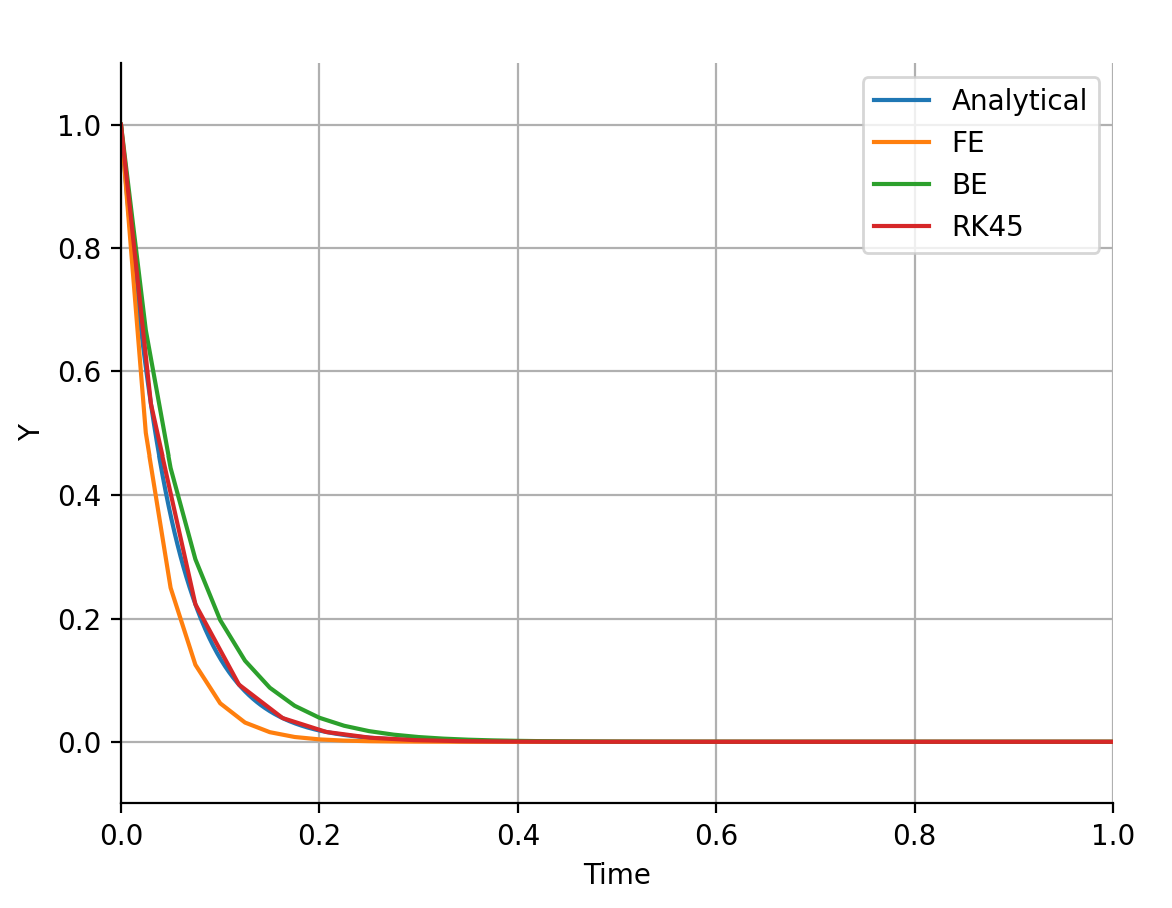
\includegraphics[width=0.7\textwidth]{RK45.png}
        \caption{Plot of the solution for $y'=-20y$ using a forward and backward Euler method as well as ‘RK45’. Additionally, it shows the analytical solution}
        \label{fig:RK45}
    \end{figure}

    \subsubsection{}
    Next the following ODE is solved using RK45 and the backward Euler method.
    Again those results are compared to the analytical solution which is also found using Python.

    \[ y'(t) = -3y(t) + 9t, \quad y(0) = 9 \]

    The analytical solution as well as the forward Euler approximation are given by:

    \[ y(t) = 3e^{-3t} + 3t \]

    and:

    \[ y_{n+1} = \frac{y_n + 9 \cdot t_{n+1} \cdot \text{{timeStep}}[n+1]}{1 + 3 \cdot \text{{timeStep}}[n+1]} \]

    \vspace{80pt}
    The code is given by:
    \begin{lstlisting}[language=Python, style=mystyle]
    ### ------------- ANALYTICAL SOLUTION -------------
    t_sym = symbols('t')
    y_sym = Function('y')
    ode = Eq(y_sym(t_sym).diff(t_sym), -3*y_sym(t_sym) + 9*t_sym)
    analytical_solution = dsolve(ode, y_sym(t_sym), ics={y_sym(0): y0})

    ### ------------- BACKWARD EULER ---------
    yBEVec = np.zeros(timeSteps)  # Allocate memory
    yBEVec[0] = y0  # Set initial condition
    # Loop over time
    for t in range(timeSteps-1):
        yBEVec[t+1] = (yBEVec[t] + 9*timeStep[t+1]*tDt) / (1 + 3*tDt)

    ### ------------- RK45 SOLVER ---------
    def odefun(t, y): return -3 * y + 9 * t
    sol = integrate.solve_ivp(odefun, [0, tStop], [y0], method='RK45')
    \end{lstlisting}

    The resulting plots are shown in Figure \ref{fig:other_function} and \ref{fig:other_function_zoom}.

    \begin{figure}[h!]
        \centering
        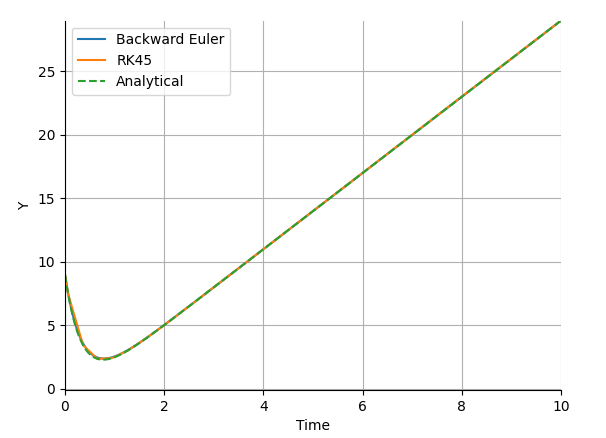
\includegraphics[width=0.7\textwidth]{other_function.png}
        \caption{Plot of the solution for $y'(t) = -3y(t) + 9t$ using a backward Euler method as well as ‘RK45’. Additionally, it shows the analytical solution}
        \label{fig:other_function}
    \end{figure}

    \begin{figure}[h!]
        \centering
        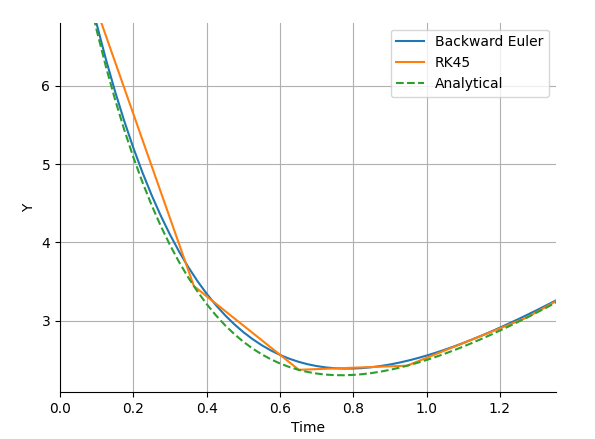
\includegraphics[width=0.7\textwidth]{other_function_zoom.png}
        \caption{Zoomed in plot of the solution for $y'(t) = -3y(t) + 9t$ using a forward and backward Euler method as well as ‘RK45’. Additionally, it shows the analytical solution}
        \label{fig:other_function_zoom}
    \end{figure}
    \clearpage

    \subsection{RC circuit / passive neuron}

    \subsubsection{}
    Looking at Figure \ref{fig:R10C0.5} - \ref{fig:R30C0.9} we can deduce the following:
    \begin{itemize}
        \item Increasing resistance (R) will lead to a higher maximal voltage.
        \item Increasing capacitance (C) will result in a slower charging and discharging of the capacitor.
    \end{itemize}

    \begin{figure}[htbp]
        \centering
        \begin{minipage}[b]{0.3\textwidth}
            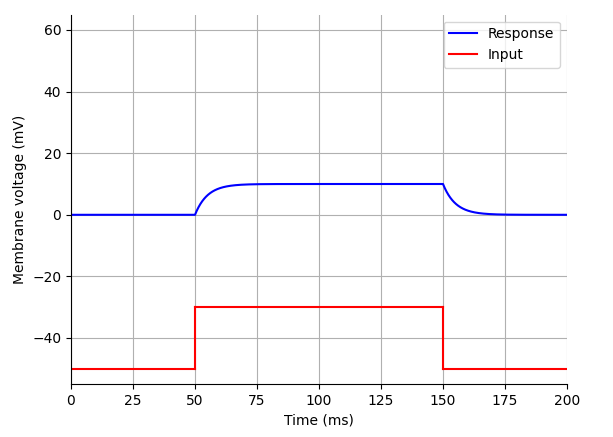
\includegraphics[width=\textwidth]{R10C0.5.png}
            \caption{Response Plot for: $R = 10 M\Omega, C = 0.5nF$}
            \label{fig:R10C0.5}
        \end{minipage}
        \hfill
        \begin{minipage}[b]{0.3\textwidth}
            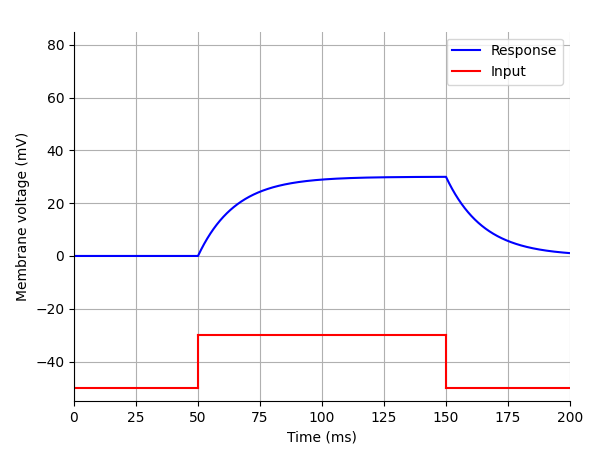
\includegraphics[width=\textwidth]{R30C0.5.png}
            \caption{Response Plot for: $R = 30 M\Omega, C = 0.5nF$}
        \end{minipage}
        \hfill
        \begin{minipage}[b]{0.3\textwidth}
            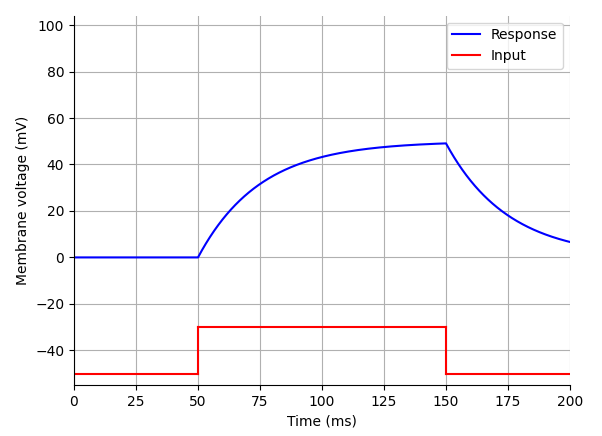
\includegraphics[width=\textwidth]{R50C0.5.png}
            \caption{Response Plot for: $R = 50 M\Omega, C = 0.5nF$}
        \end{minipage}
        \hfill
        \begin{minipage}[b]{0.3\textwidth}
            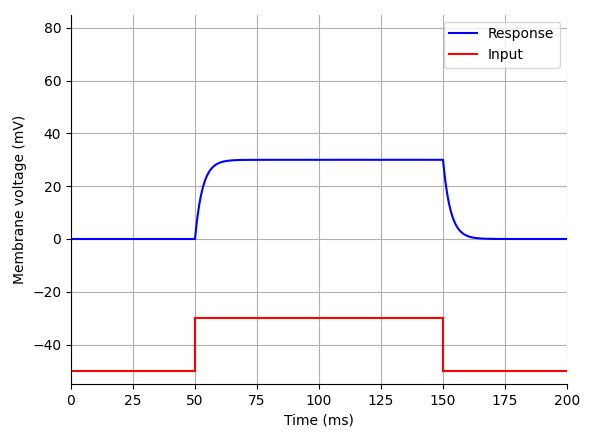
\includegraphics[width=\textwidth]{R30C0.1.png}
            \caption{Response Plot for: $R = 30 M\Omega, C = 0.1nF$}
        \end{minipage}
        \hfill
        \begin{minipage}[b]{0.3\textwidth}
        \end{minipage}
        \hfill
        \begin{minipage}[b]{0.3\textwidth}
            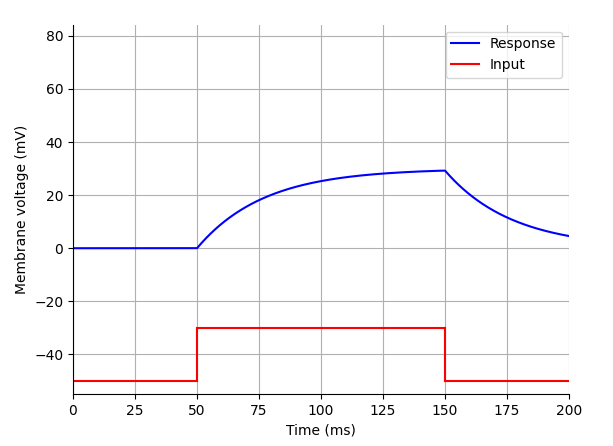
\includegraphics[width=\textwidth]{R30C0.9.png}
            \caption{Response Plot for: $R = 30 M\Omega, C = 0.9nF$}
            \label{fig:R30C0.9}
        \end{minipage}
    \end{figure}

    The time constant ($\tau$) of an RC circuit is a measure of how quickly the circuit responds to changes.
    It is given by the product of resistance ($R$) and capacitance ($C$), i.e., $\tau = R * C$.

    More specifically it is the time it takes to charge the capacitor 63.2\% of its final voltage in response to a step change in voltage.

    To find the maximum voltage in response to a current step input, we can set $\frac{dV}{dt} = 0$, giving us the equation:

    \[ 0 = -\frac{v}{R \cdot C} + \frac{I_{\text{Stim}}}{C} \]

    Solving this for $V$ gives us $V_{max}$ as:

    \[ V_{max} = I_{\text{Stim}} \cdot R \]

    The correctness of this can be easily checked by looking at the plots from Figure \ref{fig:R10C0.5} - \ref{fig:R30C0.9} (where $I_{Stim} = 1$)

    Next we calculate how long it takes until the capacitor is charged up to 99\% using.
    The voltage across a charging capacitor in an RC circuit is given by:

    \[
        v(t) = V_0 \left(1 - e^{-\frac{t}{R \cdot C}}\right)
    \]

    we can set \(v(t)\) equal to that percentage of the final value (\(V_0\)) and solve for \(t\):

    \[
        0.99 \cdot V_0 = V_0 \left(1 - e^{-\frac{t}{R \cdot C}}\right)
    \]


    \[
        0.99 = 1 - e^{-\frac{t}{R \cdot C}}
    \]

    \[
        -\frac{t}{R \cdot C} = \ln(0.01)
    \]

    Solve for \(t\):

    \[
        t = -R \cdot C \cdot \ln(0.01) \approx 4.605 \cdot R \cdot C
    \]

    Therefore, we can use factor 5 to approximate the time it takes for a capacitor to be fully charged up:
    \[
        t \approx 5 \cdot R \cdot C
    \]

    \clearpage

    \subsubsection{}
    The following code shows the implementation of the RK45 solver with the provided code as a base.
    The result is plotted together with the results of a forward and backward Euler solver and can be seen in Figure \ref{fig:RC_RK45_base}.
    The time step for the forward and backward Euler solver was set to 5ms to illustrate the differences.

    \vspace{10pt}
    Additionally, Figure \ref{fig:timestepsRK45} shows the dynamic time steps used by the RK45 solver.

    \begin{lstlisting}[language=Python, style=mystyle]
    [...]
    ### ------------- PARAMETERS ---------
    solvers = ['BE', 'FE', 'RK45']
    showTimeSteps = False
    [...]
    ### ------------- SOLVING FOR ALL SOLVERS ---------
    for solver in solvers:
            if solver != 'FE' and solver != 'BE':
                # Use scipy's solve_ivp to solve the ODE system for the built-in solver
                sol = solve_ivp(
                    lambda t, v: ode_system(t, v, I, R, C, tDel, tDur, tDt, solver),
                    [0, tStop],
                    [0],  # Initial condition
                    method=solver
                )
                # Extract the solution
                vVec_solvers[solver] = sol.y[0]
                timeSteps_solvers[solver] = sol.t
            else:
                # Solve the ODE system for Forward Euler and Backward Euler
                vVec = np.zeros(timeSteps)
                for t in range(0, timeSteps - 1):
                    IStim = 0
                    if t >= int(tDel / tDt) and t < int((tDel + tDur) / tDt):
                        IStim = I  # in nA

                    if solver == 'FE':
                        vVec[t + 1] = vVec[t] + ((-vVec[t] / R + IStim) / C) * tDt
                    elif solver == 'BE':
                        vVec[t + 1] = (vVec[t] + IStim * (tDt / C)) / (1 + tDt / (R * C))

                vVec_solvers[solver] = vVec
                timeSteps_solvers[solver] = timeStep
    [...]
    ### ------------- PLOTTING ---------
    for solver in solvers:
            plot, = ax.plot(timeSteps_solvers[solver], vVec_solvers[solver], label=solver+' Nr. Timesteps='+str(timeSteps_solvers[solver].size))
            if showTimeSteps:
                for t_step in timeSteps_solvers[solver]:
                    ax.axvline(x=t_step, color=plot.get_color(), linestyle='--', linewidth=0.8)
    [...]
    ### ------------- ODE ---------
    def ode_system(t, v, I, R, C, tDel, tDur, tDt, solver):
        # Stimulus current
        IStim = 0
        if t >= tDel and t < tDel + tDur:
            IStim = I  # in nA

        # Compute change of v
        if solver == 'BE':
            return (v + IStim * tDt / C) / (1 + tDt / (R * C))
        else:
            return (-v / R + IStim) / C
    [...]
    \end{lstlisting}

    \begin{figure}[h!]
        \centering
        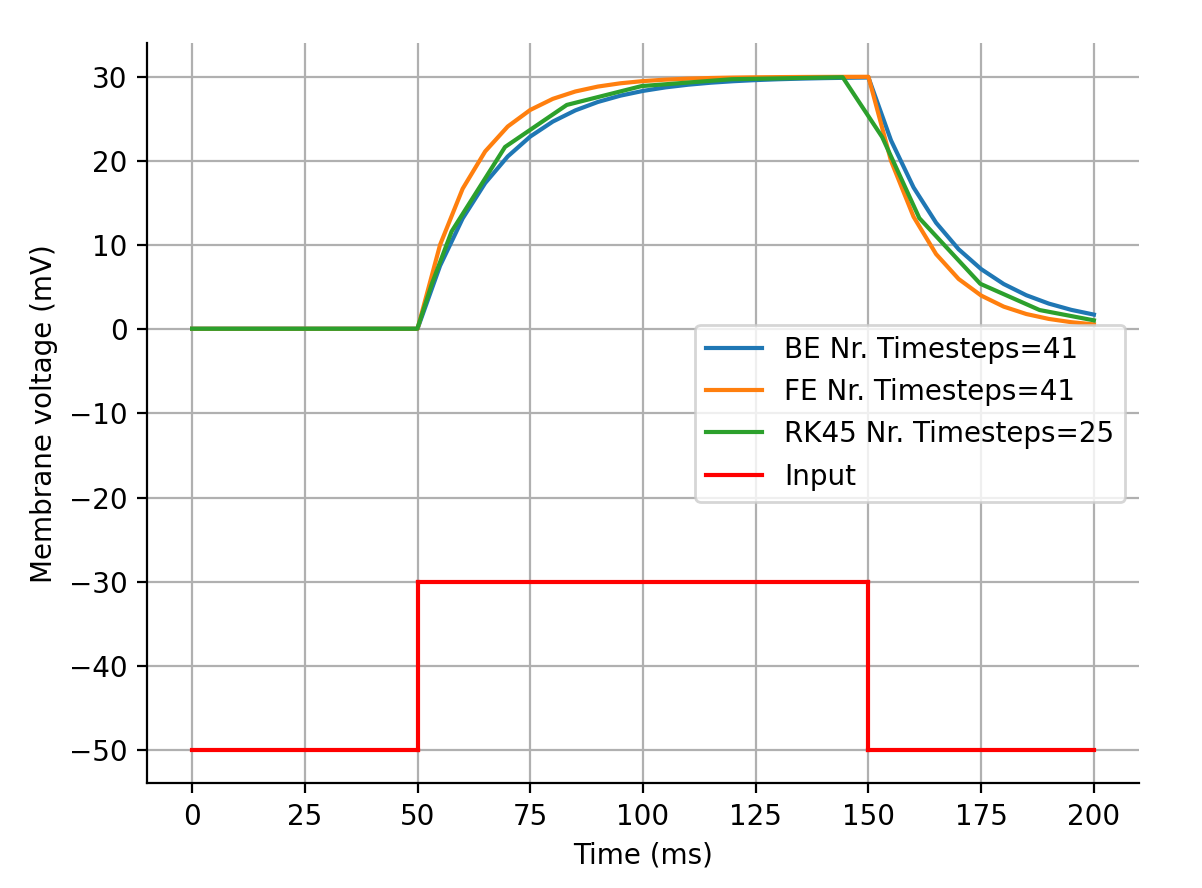
\includegraphics[width=0.7\textwidth]{RC_RK45_base.png}
        \caption{Plot of the response of an RC element calculated using a forward and backward Euler method as well as ‘RK45’}
        \label{fig:RC_RK45_base}
    \end{figure}
    \begin{figure}[h!]
        \centering
        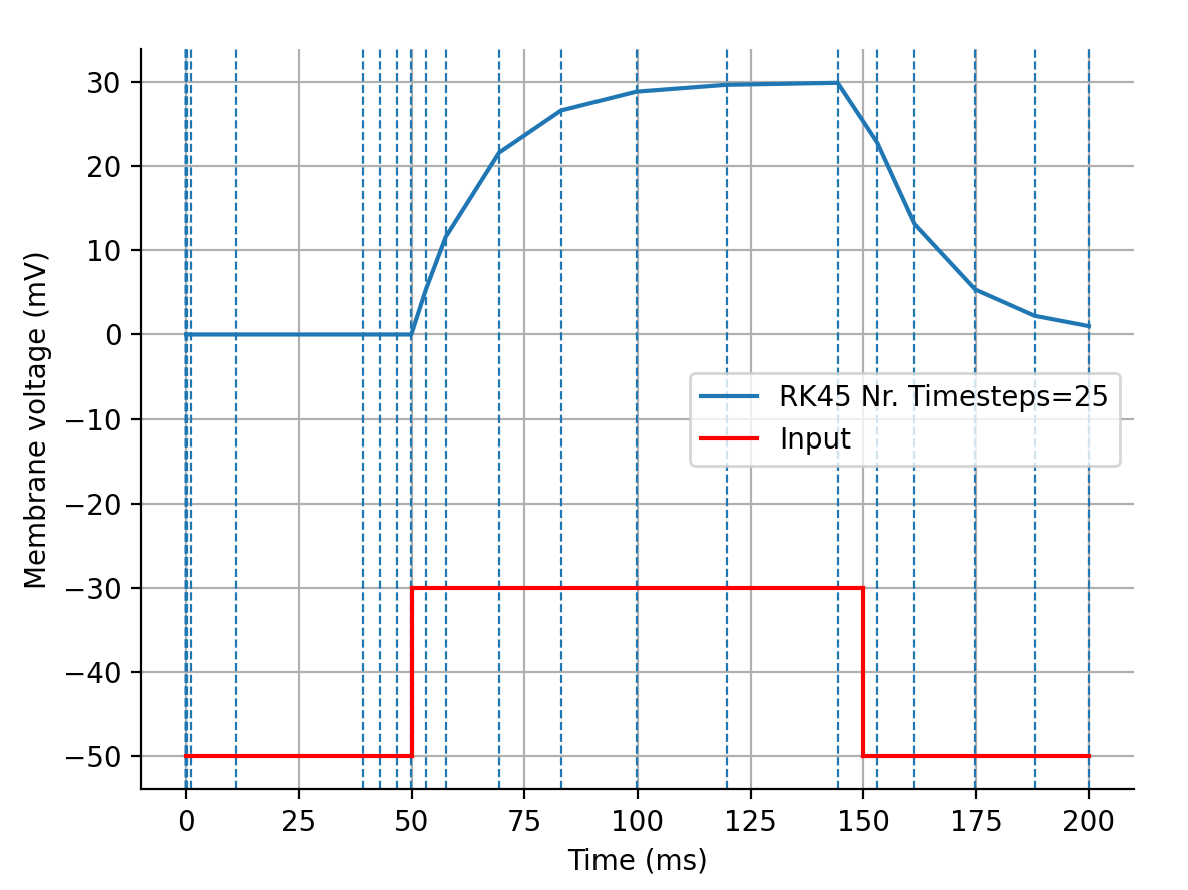
\includegraphics[width=0.7\textwidth]{timestepsRK45.png}
        \caption{Plot of the response of an RC element calculated ‘RK45’ method. The colored vertical Lines indicate the time steps made for the calculation.}
        \label{fig:timestepsRK45}
    \end{figure}
    \clearpage

    \subsubsection{}

    Using the following parameters generates the resulting plot shown in Figure \ref{fig:RC_all_solvers}.
    It gives a comparison between all the different available solvers.
    \begin{lstlisting}[language=Python, style=mystyle]
    solvers = ['RK45', 'RK23', 'DOP853', 'Radau', 'BDF', 'LSODA']
    \end{lstlisting}

    Additionally, Figure \ref{fig:RC_all_solvers_with_timesteps} shows all the dynamic time steps of those solvers (color-coded).
    The number of steps are shown in the legend.

    \vspace{10pt}
    As we can see many solvers perform better in this case than the RK45 solver.
    The issue with the solution of RK45 is, that the dip happens too early (before the dip of the input signal).

    \begin{figure}[h!]
        \centering
        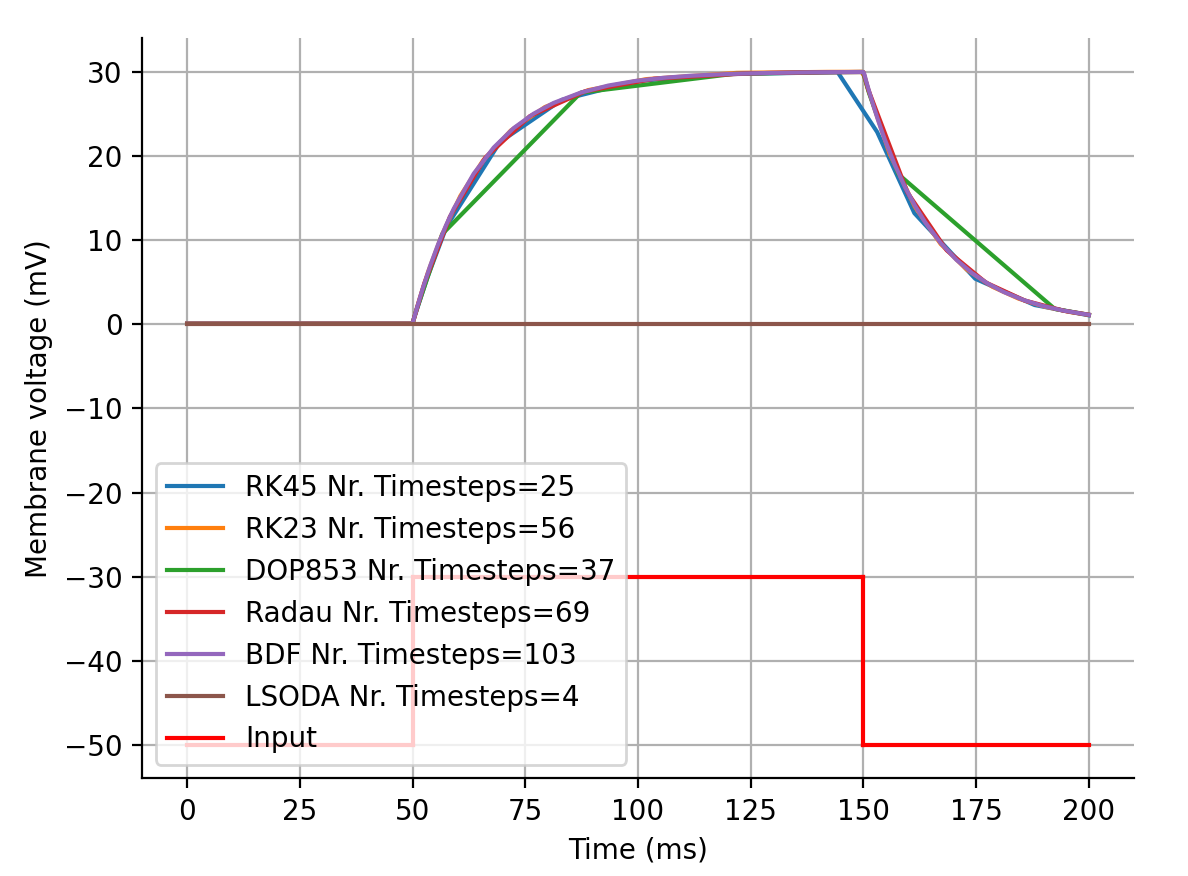
\includegraphics[width=0.7\textwidth]{RC_all_solvers.png}
        \caption{Plot of the response of an RC element calculated using a forward and backward Euler method as well as ‘RK45’}
        \label{fig:RC_all_solvers}
    \end{figure}
    \begin{figure}[h!]
        \centering
        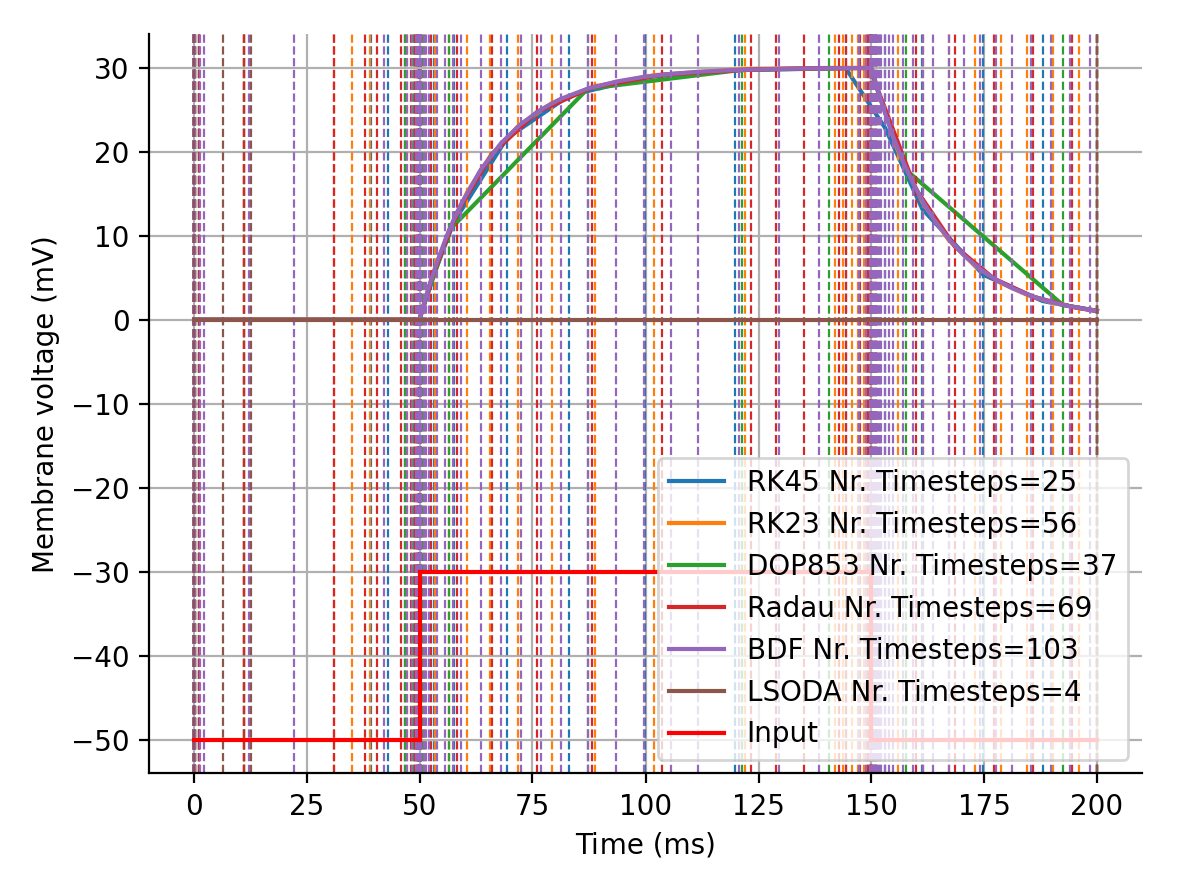
\includegraphics[width=0.7\textwidth]{RC_all_solvers_with_timesteps.png}
        \caption{Plot of the response of an RC element calculated ‘RK45’ method. The colored vertical Lines indicate the time steps made for the calculation.}
        \label{fig:RC_all_solvers_with_timesteps}
    \end{figure}

    \vspace{10pt}
    Figure \ref{fig:RK45_vs_RK23} shows a comparison between RK45 and RK23.
    In this specific case the RK23 solver actually performs better than the RK45 solver, since its closer to the real solution. It also uses more time steps though.

    \vspace{10pt}
    A second example of a better-performing solver is the Radau solver shown in Figure \ref{fig:RK45_vs_Radau}.
    It is intended to be used with stiff ODEs which our ODE can be classified as, at least to a degree.
    Radau however also uses almost three times the time steps compared to RK45.
    \begin{figure}[h!]
        \centering
        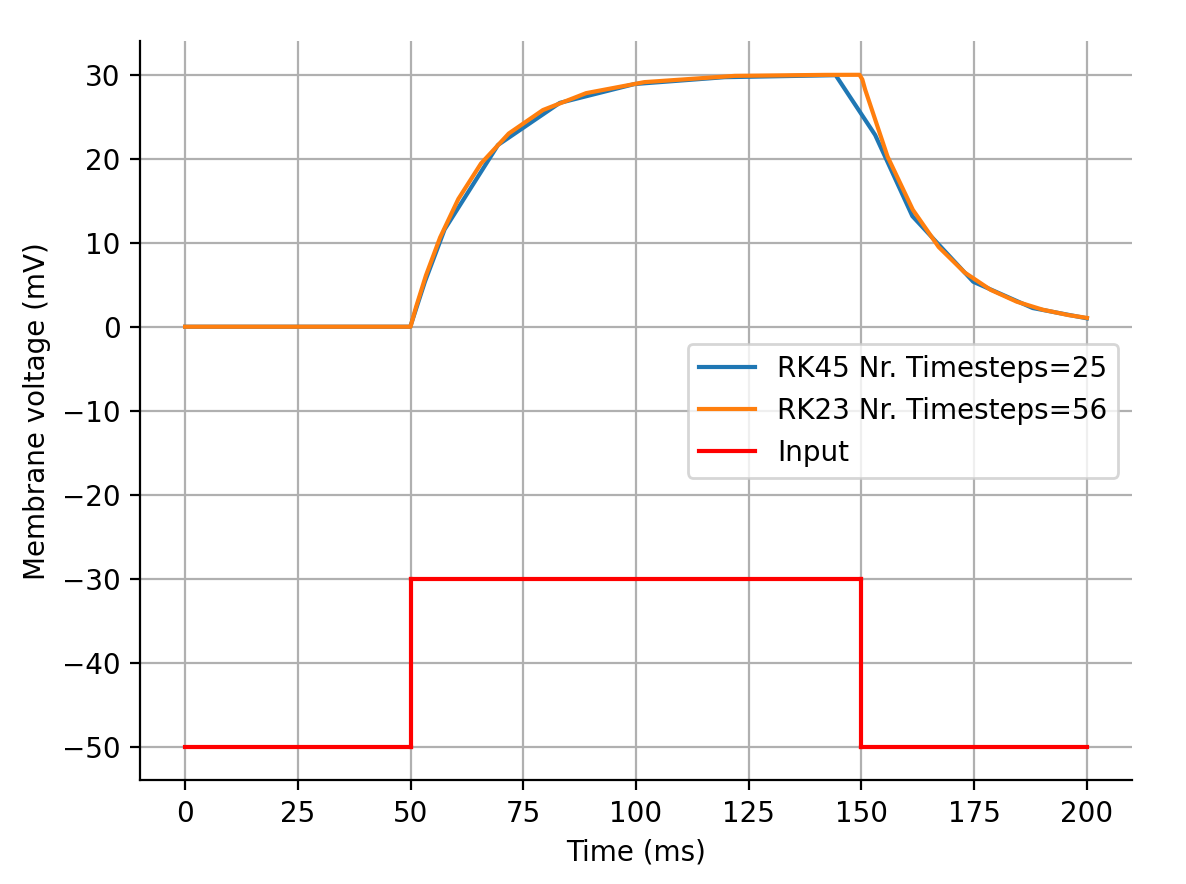
\includegraphics[width=0.7\textwidth]{RK45_vs_RK23.png}
        \caption{Plot of the response of an RC element calculated ‘RK45’ method. The colored vertical Lines indicate the time steps made for the calculation.}
        \label{fig:RK45_vs_RK23}
    \end{figure}
    \begin{figure}[h!]
        \centering
        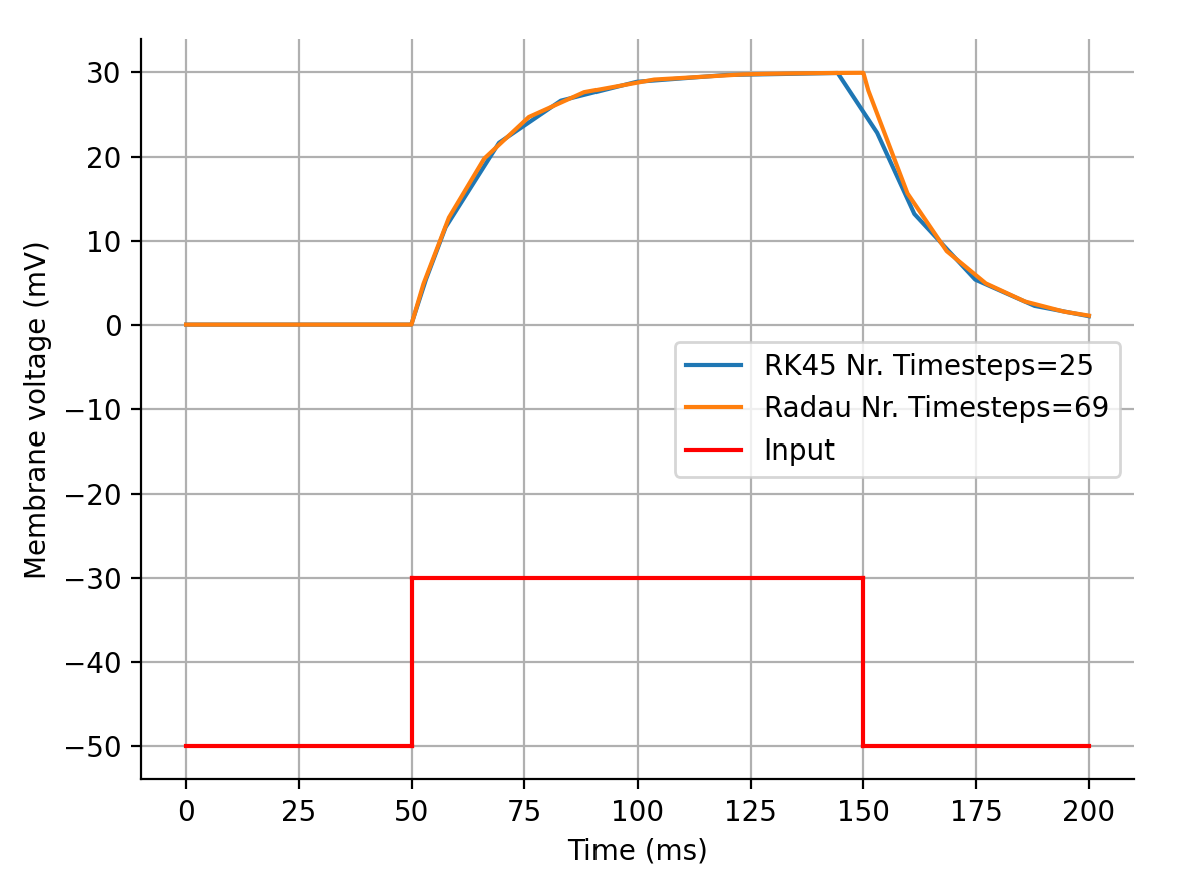
\includegraphics[width=0.7\textwidth]{RK45_vs_Radau.png}
        \caption{Plot of the response of an RC element calculated ‘RK45’ method. The colored vertical Lines indicate the time steps made for the calculation.}
        \label{fig:RK45_vs_Radau}
    \end{figure}

    \clearpage

    \subsubsection{}
    We can also try to 'tune' the RK45 solver in order to get better results.
    For this we can for example use the relative and absolute tolerances ($r_{tol}$ and $a_{tol}$).

    Figure \ref{fig:timestepsRK45-2} - \ref{fig:RK45_tuned} show a comparison between the results of the untuned and the tuned version of the RK45 solver with $r_{tol} = 5 \cdot 10^{-5}$ and $a_{tol} = 5 \cdot 10^{-7}$

    \vspace{10pt}
    As we can see, we can eliminate the early dip using those parameter values while still keeping a low amount of time steps.
    The lower we choose those parameter values the more time steps we will have and the more accurate are result will become.

    \begin{figure}[htbp]
        \centering
        \begin{minipage}[b]{0.49\textwidth}
            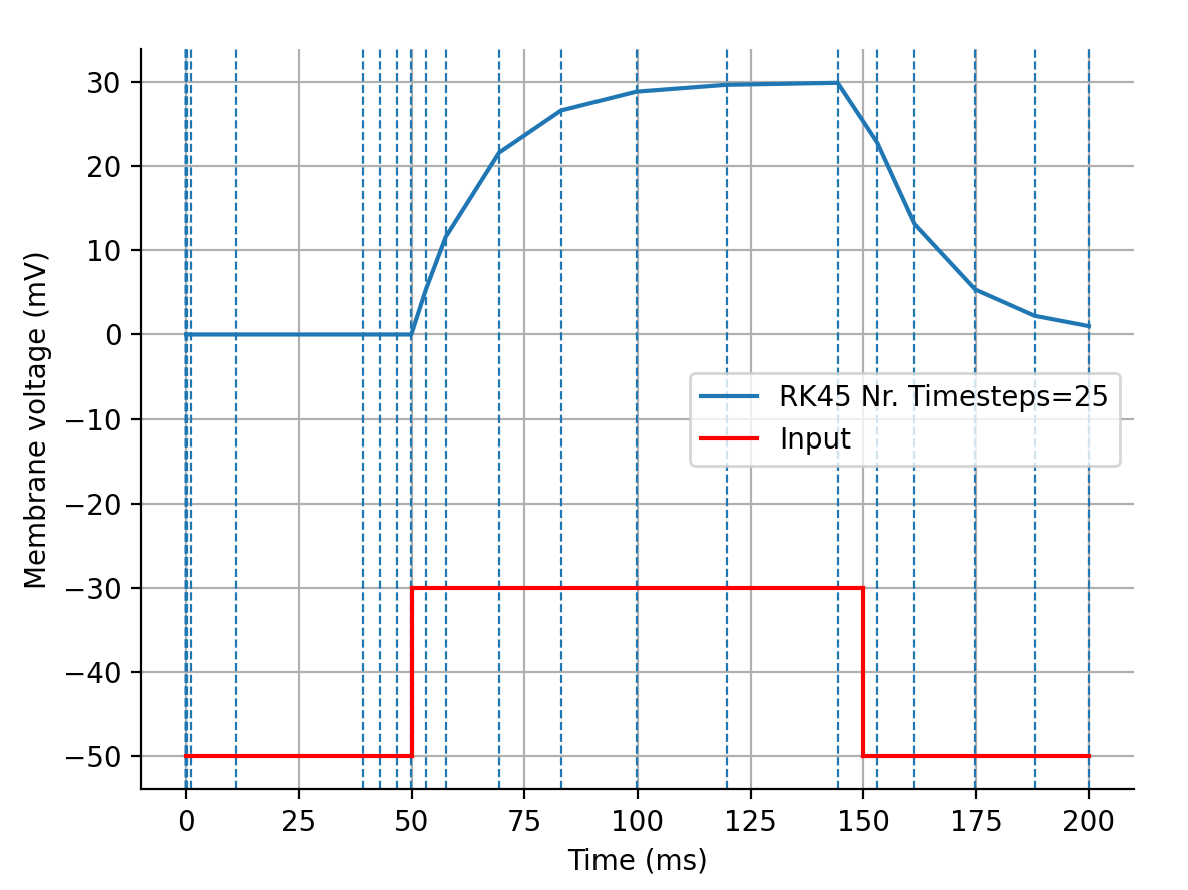
\includegraphics[width=\textwidth]{timestepsRK45.png}
            \caption{Response Plot of the RK45 solver with default parameters}
            \label{fig:timestepsRK45-2}
        \end{minipage}
        \hfill
        \begin{minipage}[b]{0.49\textwidth}
            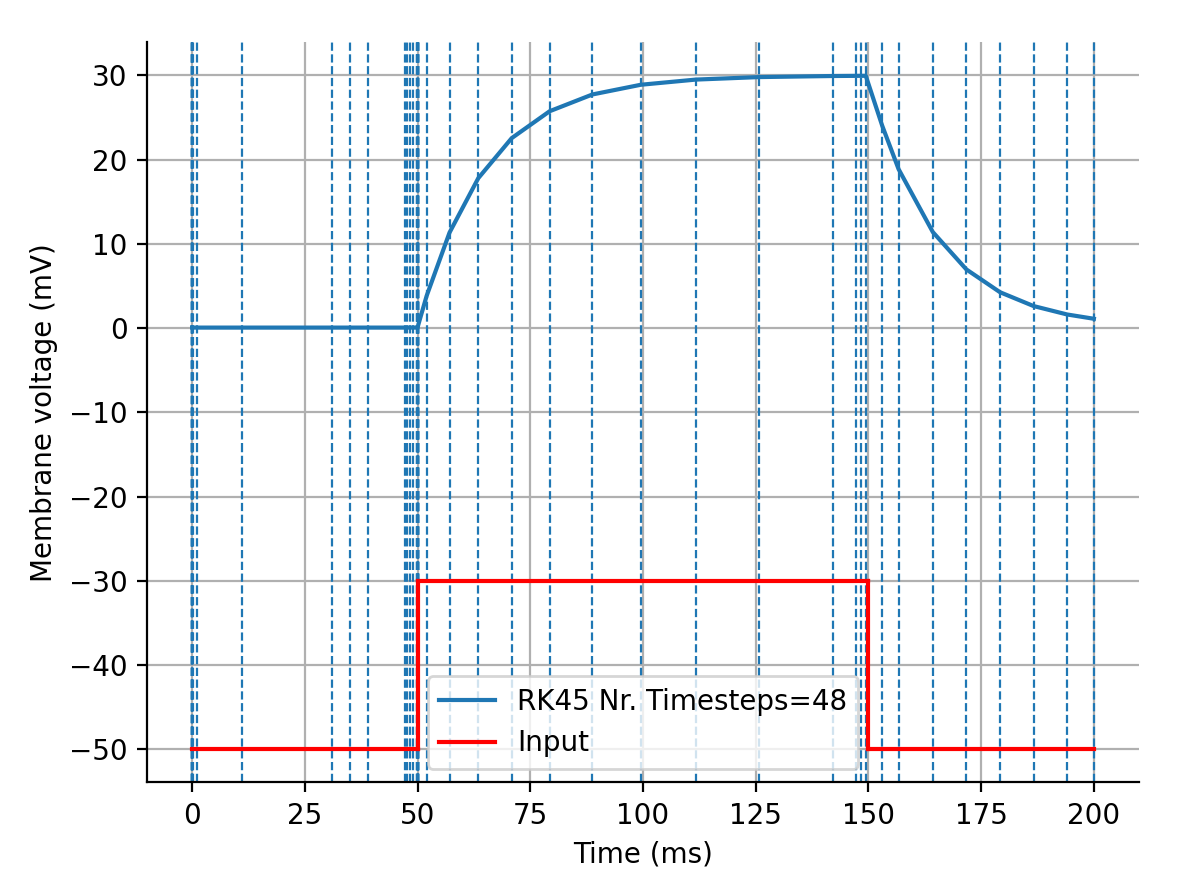
\includegraphics[width=\textwidth]{RK45_tuned.png}
            \caption{Response Plot of the RK45 solver with $r_{tol} = 5 \cdot 10^{-5}$ and $a_{tol} = 5 \cdot 10^{-7}$}
            \label{fig:RK45_tuned}
        \end{minipage}
    \end{figure}


    \section{Hodgkin-Huxley Model (single)}

    \subsection{}

    When varying the amplitude of the applied stimulus ($I$) for a $0.5$ ms long pulse, we find, that the threshold current is at around $13.45 uA/cm^2$
    The resulting action potential can be seen in Figure \ref{fig:threshold_amplitudes}.

    \begin{figure}[htbp]
        \centering
        \begin{minipage}[b]{0.49\textwidth}
            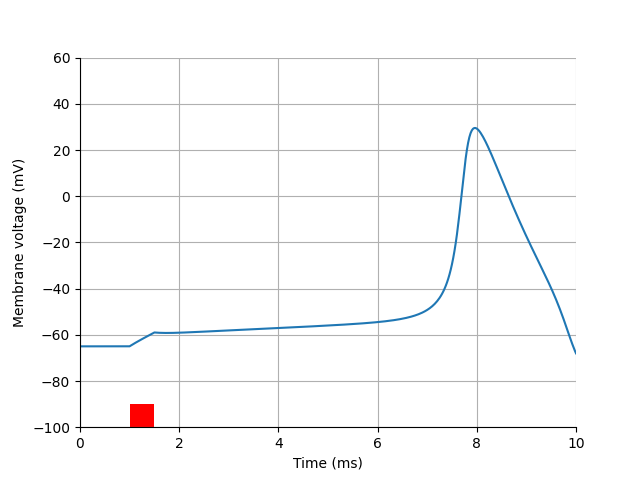
\includegraphics[width=\textwidth]{threshold(13.45).png}
            \caption{Membrane voltage over time for the spiking threshhold.}
            \label{fig:threshold_amplitudes}
        \end{minipage}
        \hfill
        \begin{minipage}[b]{0.49\textwidth}
            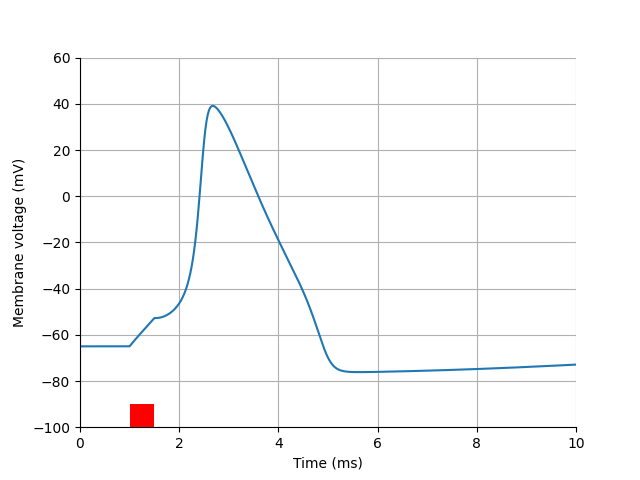
\includegraphics[width=\textwidth]{double_threshold(26.9).png}
            \caption{Membrane voltage over time for double the spiking threshhold.}
            \label{fig:double_threshold_amplitudes}
        \end{minipage}
    \end{figure}

    When the stimulus amplitude is doubled ($I = 26.9$ $\mu A/cm^2$), the action potential is initiated earlier.
    The resulting plot can be seen in Figure \ref{fig:double_threshold_amplitudes}

    \subsection{}

    As we can see in Figure \ref{fig:ac_backward_euler} and \ref{fig:ac_forward_euler}, when increasing the time step to $tDt = 0.1 ms$ and $I = 20\mu A/cm^2$ we still get a good solution with the Backward Euler Solver.
    The Forward Euler however produces immense oscillations, indicating that the time step is to big for this solver.
    The reason why this happens was discussed in a previous section.

    \begin{figure}[htbp]
        \centering
        \begin{minipage}[b]{0.49\textwidth}
            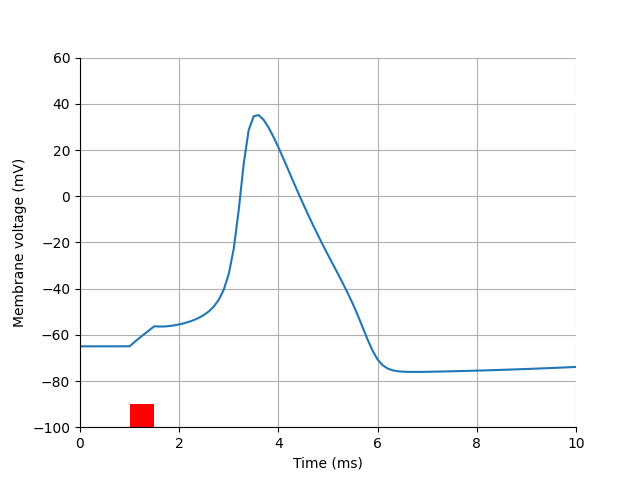
\includegraphics[width=\textwidth]{ac_backward_euler}
            \caption{Action potential response solved with the Backward Euler Method}
            \label{fig:ac_backward_euler}
        \end{minipage}
        \hfill
        \begin{minipage}[b]{0.49\textwidth}
            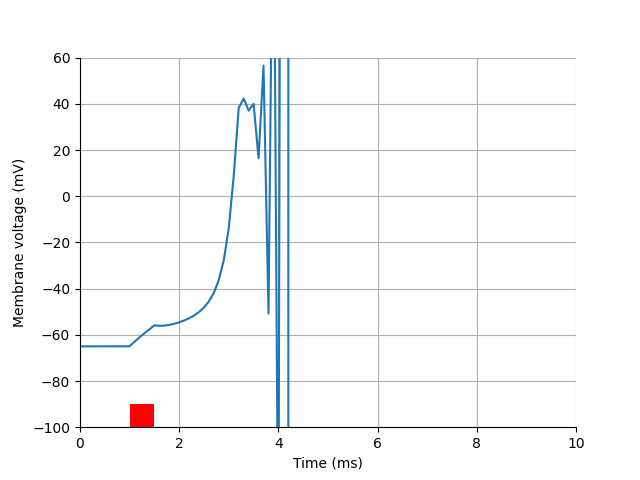
\includegraphics[width=\textwidth]{ac_forward_euler}
            \caption{Action potential response solved with the Forward Euler Method}
            \label{fig:ac_forward_euler}
        \end{minipage}
    \end{figure}

    \subsection{}

    Figure \ref{fig:membrane_voltage_currents} illustrates the behavior of the membrane voltage and the sodium and potassium current densities during the simulation.
    The code that produced this plot it given by:

    \begin{lstlisting}[language=Python, style=mystyle]
    fig, ax1 = plt.subplots()
    ax1.grid()
    ax1.set_xlabel('Time (ms)')
    ax1.set_ylabel('Membrane voltage (mV)', color='tab:blue')
    ax1.plot(timeStep, vVec, label='Membrane Voltage', color='tab:blue')
    ax1.tick_params(axis='y', labelcolor='tab:blue')

    ax2 = ax1.twinx()  # instantiate a second axes that shares the same x-axis
    ax2.set_ylabel('Current densities (uA/cm2)', color='tab:red')

    # Plot sodium and potassium current densities with legends
    ax2.plot(timeStep, gNa * mVec**3 * hVec * (vVec - eNa), '--', label='Sodium Current (iNa)', color='tab:red')
    ax2.plot(timeStep, gK * nVec**4 * (vVec - eK), '-.', label='Potassium Current (iK)', color='tab:green')

    ax2.tick_params(axis='y', labelcolor='tab:red')

    # Add legend
    lines, labels = ax1.get_legend_handles_labels()
    lines2, labels2 = ax2.get_legend_handles_labels()
    ax2.legend(lines + lines2, labels + labels2, loc='upper right')

    fig.tight_layout()  # ensure the shared x-axis labels are not slightly cut off
    plt.show()
    \end{lstlisting}

    \begin{figure}[h]
        \centering
        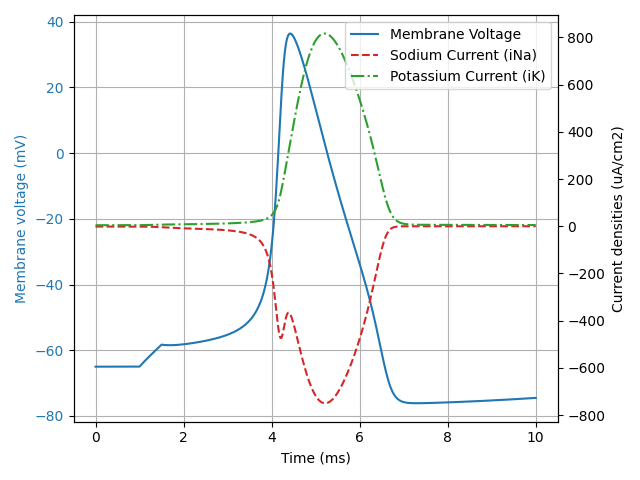
\includegraphics[width=0.7\textwidth]{channel_activation.png}
        \caption{Membrane voltage and current densities over time. ($I = 15 \mu A/cm^2$, $tDur = 0.5 ms$)}
        \label{fig:membrane_voltage_currents}
    \end{figure}

    The rise in the membrane voltage during the initial phase of the simulation is caused by the influx of sodium ions through voltage-gated sodium channels.
    This depolarization phase is a result of the activation of sodium channels (governed by variables $m$ and $h$) and the subsequent increase in sodium current density.
    After reaching a peak, the membrane voltage starts to decline due to the inactivation of sodium channels and the activation of potassium channels.
    The potassium current density increases, leading to repolarization and the restoration of the resting membrane voltage.

    \subsection{}
    As can be seen in Figure \ref{fig:ac_at_2degree} and \ref{fig:ac_at_10degree} higher temperatures generally lead to shorter action potential durations (widths) and decreased action potential amplitudes (heights).
    The peak tends to appear earlier for higher temperatures.

    \begin{figure}[htbp]
        \centering
        \begin{minipage}[b]{0.49\textwidth}
            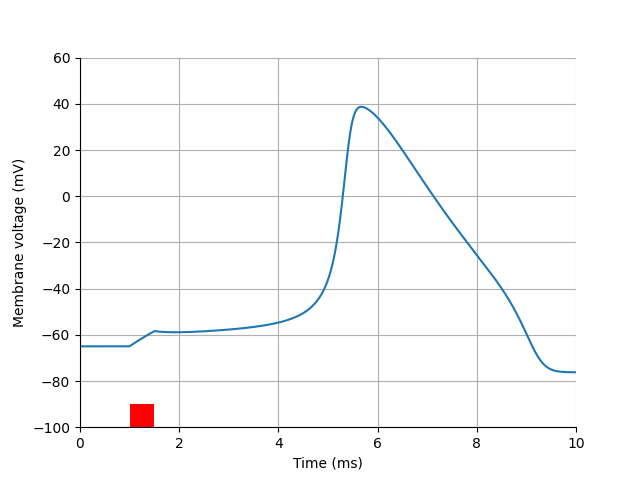
\includegraphics[width=\textwidth]{ac_at_2degree.png}
            \caption{Action Potential at 2°C}
            \label{fig:ac_at_2degree}
        \end{minipage}
        \hfill
        \begin{minipage}[b]{0.49\textwidth}
            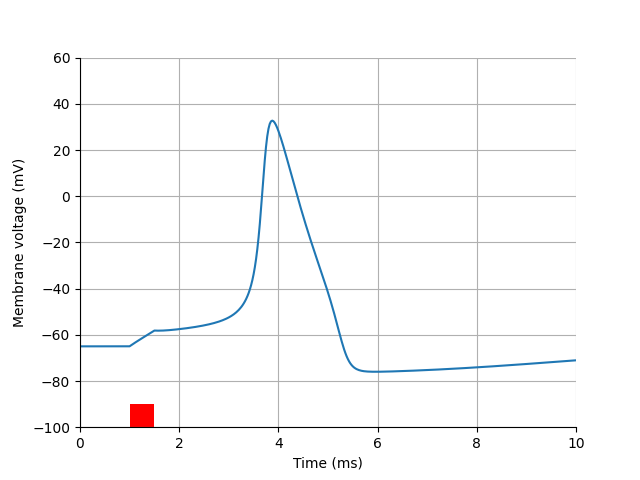
\includegraphics[width=\textwidth]{ac_at_10degree.png}
            \caption{Action Potential at 10°C}
            \label{fig:ac_at_10degree}
        \end{minipage}
    \end{figure}

    For temperatures above 15\°C we can no longer observe an action potential.
    This also means that with the previously chosen parameters we do not get am action potential at 37\°C.
    Still it has been shown many times be researcher, that the Hodgkin-Huxley model can be used for humans.
    For this we would have to adapt our parameters accordingly, though.

    \subsection{}
    The sodium current density (\(i_{Na}\)) in the Hodgkin \& Huxley model is given by the equation:

    \[ i_{Na} = g_{Na} \cdot m^3 \cdot h \cdot (v - e_{Na}) \]

    where:
    \begin{align*}
        g_{Na} & : \text{Sodium channel maximum conductivity} \\
        m & : \text{Activation gating variable} \\
        h & : \text{Inactivation gating variable} \\
        v & : \text{Membrane voltage} \\
        e_{Na} & : \text{Sodium reversal/equilibrium potential}
    \end{align*}

    The conditions under which the sodium flux reverses its direction, leading to a repolarizing effect, occur when the membrane voltage exceeds the sodium reversal potential (\(e_{Na}\)).

    \vspace{10pt}
    The activation gating variable \(m\) responds to an increase in membrane voltage by increasing its value.
    The equation governing \(m\) in the model is:

    \[ \frac{dm}{dt} = \alpha_m \cdot (1 - m) - \beta_m \cdot m \]

    where:
    \begin{align*}
        \alpha_m & : \text{Rate of activation} \\
        \beta_m & : \text{Rate of deactivation}
    \end{align*}

    An increase in membrane voltage generally leads to an increased activation of sodium channels, resulting in an increase in \(m\) and a higher probability of sodium channels being open.

    \vspace{10pt}
    The inactivation gating variable \(h\) responds to an increase in membrane voltage by decreasing its value.
    The equation governing \(h\) in the model is:

    \[ \frac{dh}{dt} = \alpha_h \cdot (1 - h) - \beta_h \cdot h \]

    where:
    \begin{align*}
        \alpha_h & : \text{Rate of inactivation} \\
        \beta_h & : \text{Rate of deinactivation}
    \end{align*}

    An increase in membrane voltage typically leads to a decrease in the inactivation of sodium channels, resulting in a decrease in \(h\) and a lower probability of sodium channels being inactivated.

    \subsection{}

    The following Python script computes the Strength-Duration (SD) curve for the single-compartment Hodgkin \& Huxley model.
    The script uses a binary search algorithm to efficiently find the threshold for different pulse durations.

    \begin{lstlisting}[language=Python, style=mystyle]
    def binary_search_threshold(time_step, stim_duration, pulse_amplitude):
        low, high = 0, 1000  # Initial search range for threshold
        threshold = None

        while high - low > 1e-6:
            current_amplitude = (low + high) / 2
            _, v, _, _, _ = HH_single(I=current_amplitude, tDur=stim_duration)
            max_voltage = np.max(v)

            if max_voltage > 0:
                high = current_amplitude
                threshold = current_amplitude
            else:
                low = current_amplitude

        return threshold
    [...]

    # Parameters
    pulse_durations = np.logspace(-2, 2, 20)  # Pulse durations from 0.01 to 100 ms in 20 logarithmic steps
    stim_duration_long_pulse = 100  # Duration of the long pulse for rheobase calculation

    # Compute SD curve
    thresholds = []

    for duration in pulse_durations:
        threshold = binary_search_threshold(0.025, duration, 15)
        thresholds.append(threshold)
    [...]

    rheobase = binary_search_threshold(0.025, stim_duration_long_pulse, 15)
    double_rheobase = 2 * rheobase
    index_double_rheobase = np.argmin(np.abs(np.array(thresholds) - double_rheobase))
    chronaxie = pulse_durations[index_double_rheobase]
    \end{lstlisting}

    \begin{figure}[h]
        \centering
        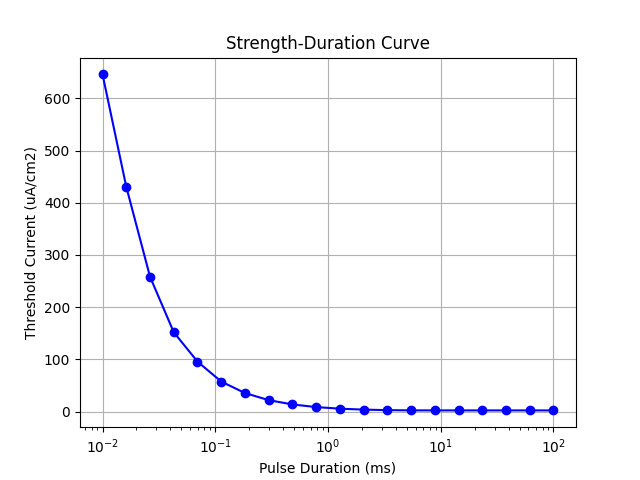
\includegraphics[width=0.8\textwidth]{sd_curve.png}
        \caption{Strength-Duration Curve for the Hodgkin \& Huxley Model.}
        \label{fig:sd_curve_plot}
    \end{figure}

    From the computed SD curve we get the following values for the Rheobase and Chronaxie:

    \begin{itemize}
        \item Rheobase: 2.22 uA/cm\textsuperscript{2}
        \item Chronaxie: 2.07 ms
    \end{itemize}

    \subsection{}


    The following Python script computes the spiking probability for amplitudes between 0 and 30 $\mu A/cm^2$.
    For each amplitude, the simulation is run 50 times, and a logistic curve is fitted to the simulated data.

    \begin{lstlisting}[language=Python, style=mystyle]
    def logistic_function(x, L, k, x0):
        return L / (1 + np.exp(-k * (x - x0)))

    # Parameters
    amplitudes = np.arange(0, 30, 1)  # Stimulus amplitudes from 0 to 30 μA/cm² in 1 μA/cm² steps
    num_simulations = 50
    tDur = 0.5

    # Function to run simulation and compute spiking probability
    def run_simulation_and_compute_probability(amplitude):
        spiking_count = 0

        for _ in range(num_simulations):
            _, v, _, _, _ = HH_single(I=amplitude, tDur=tDur)
            if np.max(v) > 0:
                spiking_count += 1

        spiking_probability = spiking_count / num_simulations * 100
        return spiking_probability

    # Compute spiking probabilities
    spiking_probabilities = [run_simulation_and_compute_probability(amplitude) for amplitude in amplitudes]

    # Fit a logistic curve to the spiking probabilities
    params, _ = curve_fit(logistic_function, amplitudes, spiking_probabilities, p0=[100, 1, 15])
    \end{lstlisting}

    Additionally, a random factor is added to the total ionic current:
    \begin{lstlisting}[language=Python, style=mystyle]
    iIon = iNa+iK+iL + 20 * np.random.randn() # in uA/cm2
    \end{lstlisting}

    \begin{figure}[h]
        \centering
        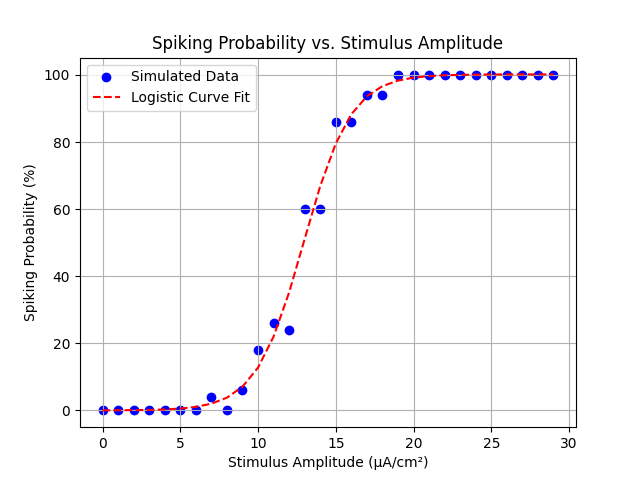
\includegraphics[width=0.8\textwidth]{spiking_probability.png}
        \caption{Spiking Probability vs. Stimulus Amplitude with Logistic Curve Fit.}
        \label{fig:spiking_probability_plot}
    \end{figure}

    The resulting plot can be seen in Figure \ref{fig:spiking_probability_plot} and the parameters of the fitted logistic curve are:

    \begin{itemize}
        \item Parameter \(L\): 100.18
        \item Parameter \(k\): 0.66
        \item Parameter \(x_0\): 12.94
    \end{itemize}


    \section{Multi-Compartment Hodgkin-Huxley Model}

    \subsection{}
    The membrane voltage was for a stimulation current of \( I = -0.5 \muA \) plotted over the location of the fiber at a specific timestamp, which was chosen to be 0.1 ms after the stimulus onset.
    The resultant plot is shown in Figure \ref{fig:membrane_voltage}.

    \vspace{10pt}
    The code that produces the plot is given by:

    \begin{lstlisting}[language=Python, style=mystyle]
    specific_timestamp = int((tDel + 0.1) / tDt)
    fig, ax = plt.subplots()
    location = np.arange(-lComp * (nComp // 2), lComp * (nComp // 2) + 1, lComp)
    ax.plot(location, vMat[:, specific_timestamp], 'b')
    ax.set_xlabel('Location along fiber (μm)')
    ax.set_ylabel('Membrane Voltage (mV)')
    ax.set_title('Membrane Voltage Distribution at t = {:.2f} ms'.format(specific_timestamp * tDt))
    plt.show()
    \end{lstlisting}

    \begin{figure}[h]
        \centering
        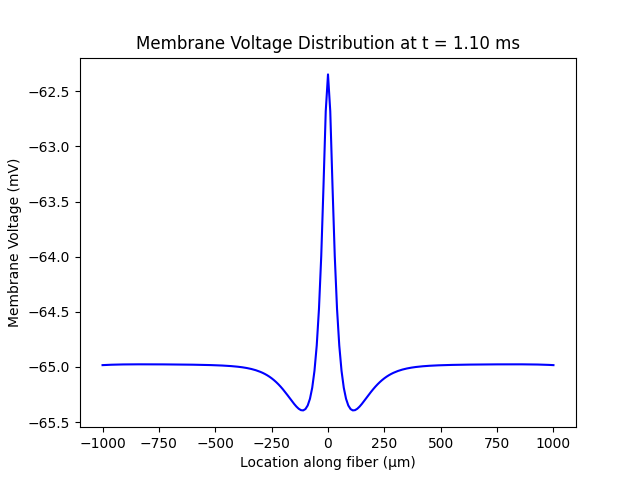
\includegraphics[width=0.8\textwidth]{membrane_voltage}
        \caption{Membrane voltage distribution along the fiber at a specific time point after the onset of the cathodic stimulus.}
        \label{fig:membrane_voltage}
    \end{figure}

    \vspace{10pt}
    When a cathodic stimulus is applied, the area immediately beneath the electrode becomes hyperpolarized due to the influx of negative charges.
    This creates a local potential difference between the stimulated area and adjacent regions.
    Adjacent regions experience a relative depolarization due to this, as positive charges flow towards the hyperpolarized area to balance the potential.

    \subsection{}
    The activating function is calculated as the second spatial derivative of the extracellular potential and plotted using the following code:

    \begin{lstlisting}[language=Python, style=mystyle]
    fig, ax = plt.subplots()
    location = np.arange(-lComp * (nComp // 2), lComp * (nComp // 2) + 1, lComp)
    ax.plot(location, np.gradient(np.gradient(potentials)), 'b')
    plt.title('Activating Function for Cathodic Pulse')
    plt.xlabel('Location along fiber (μm)')
    plt.ylabel('Activating Function (mV/ms)')
    plt.show()
    \end{lstlisting}

    \begin{figure}[htbp]
        \centering
        \begin{minipage}[b]{0.49\textwidth}
            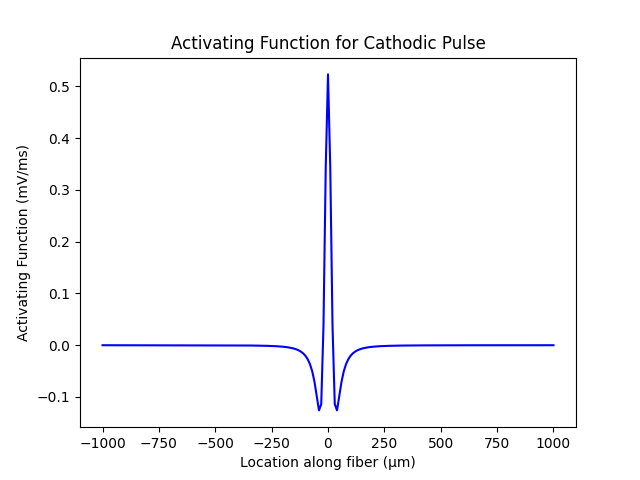
\includegraphics[width=\textwidth]{activating_function_cathodic.png}
            \caption{Activating functions for a cathodic pulse.}
            \label{fig:activating_function_cathodic}
        \end{minipage}
        \hfill
        \begin{minipage}[b]{0.49\textwidth}
            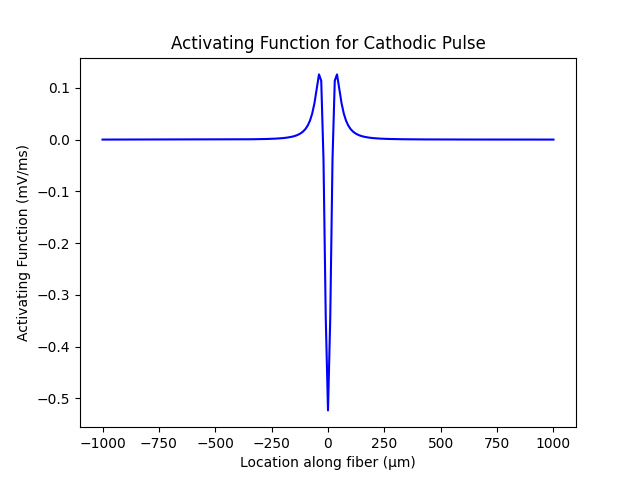
\includegraphics[width=\textwidth]{activating_function_anodic.png}
            \caption{Activating functions for an anodic pulse}
            \label{fig:activating_function_anodic}
        \end{minipage}
    \end{figure}

    As can be seen in Figure~\ref{fig:activating_function_cathodic} and~\ref{fig:activating_function_anodic}, the activation function shows the regions that have high probability of hyperpolarization or depolarization in a given electric field.
    The cathodic and anodic activation functions are the inverse of each other, which is in alignment with the fact, that a positive stimulus can induce a hyperpolarization at the exact position where a negative stimulus can induce a depolarization.

    \subsection{}
    Using the previous parameters of our model and altering the Stimulus amplitude, we find, that cathodic threshold to initiate an action potential from a point source is \(I = -4\mu A\) and for a disk with \(d = 50\mu m\) the threshold is \(I = -2.5\mu A\).
    The action potential is initiated at the center, directly underneath the electrode and propagates outwards to the left and right from there.
    This can be seen in Figure \ref{fig:threshold_point} and \ref{fig:threshold_disk}.

    \begin{figure}[htbp]
        \centering
        \begin{minipage}[b]{0.49\textwidth}
            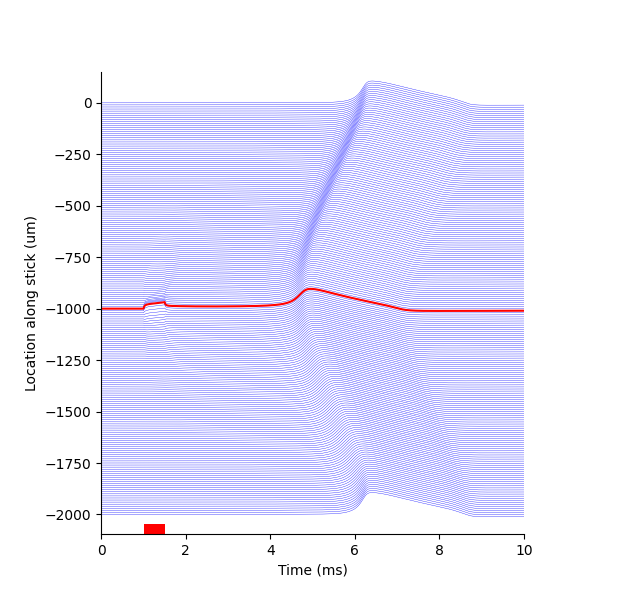
\includegraphics[width=\textwidth]{threshold_point}
            \caption{Propagating action potential initiated from a point electrode}
            \label{fig:threshold_point}
        \end{minipage}
        \hfill
        \begin{minipage}[b]{0.49\textwidth}
            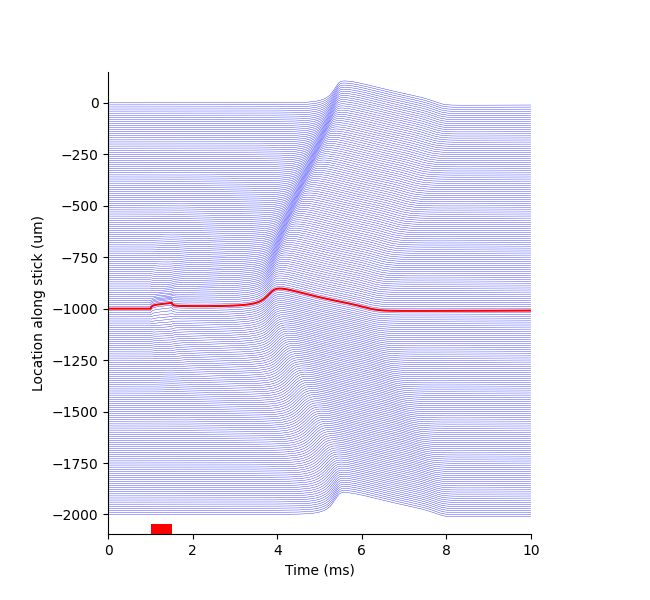
\includegraphics[width=\textwidth]{threshold_disk}
            \caption{Propagating action potential initiated from a disk electrode}
            \label{fig:threshold_disk}
        \end{minipage}
    \end{figure}

    \subsection{}
    When the intracellular resistivity increases, it becomes harder for the ionic currents to flow through the cytoplasm within the axon.
    This increased resistance slows down the rate at which the depolarization spreads down the axon.
    Decreasing the intracellular resistivity on the other hand increases the conduction velocity of an action potential.

    \subsection{}
    Despite initial hyperpolarization, it is still possible to trigger an action potential with an anodic pulse at higher amplitudes.
    This phenomenon is known as anodal break excitation.
    After the end of the anodic pulse, there can be a rebound effect.
    The membrane potential, having been hyperpolarized, returns to its resting state.
    This rebound can overshoot, leading to depolarization sufficient to reach the threshold for an action potential.
    For anodic stimulation, the action potential is typically not initiated directly under the electrode (where the hyperpolarization is greatest) but rather at a location adjacent to this area.

    \subsection{}
    The following code was used to create the spiking activity plot that can be seen in Figure \ref{fig:spiking_activity}:

    \begin{lstlisting}[language=Python, style=mystyle]
    def detect_spiking(vMat):
        threshold = -20  # Threshold voltage for spiking in mV
        return 1 if np.any(vMat > threshold) else 0

    def HH_multi(cellX):

        [...]

        I = -5
        cellY = 25

        [...]

        return detect_spiking(vMat)

    if __name__ == '__main__':
        cellX_values = np.arange(-3000, 3001, 100)  # cellX from -3000 to 3000 in steps of 100 µm
        spiking_activity = []

        for cellX in cellX_values:
            spiking = HH_multi(cellX)
            spiking_activity.append(spiking)

        # Plotting spiking activity vs. cellX coordinate
        plt.plot(cellX_values, spiking_activity, 'o-')
        plt.xlabel('Cell X Coordinate (µm)')
        plt.ylabel('Spiking Activity (0=No, 1=Yes)')
        plt.title('Spiking Activity vs. Cell X Coordinate')
        plt.grid(True)
        plt.show()
    \end{lstlisting}

    \begin{figure}[h]
        \centering
        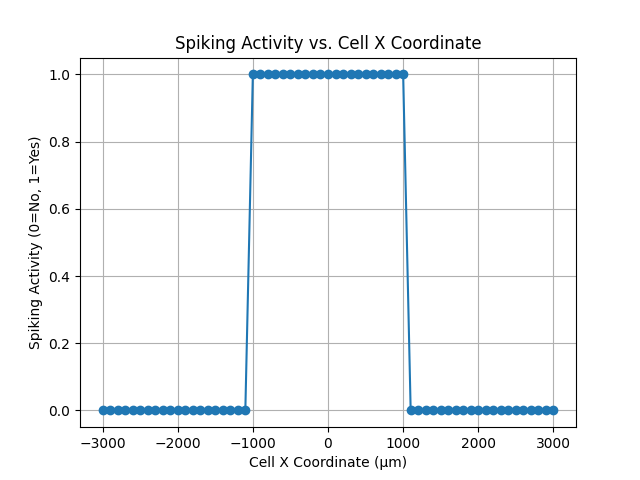
\includegraphics[width=0.8\textwidth]{spiking_activity}
        \caption{Spiking activity for a shifting electrode along the fiber}
        \label{fig:spiking_activity}
    \end{figure}


    \section{Finite Element Simulation}

    \subsection{}

    Figures \ref{fig:FE_structure}-\ref{fig:FE_efield_1} show the configuration built in \texttt{Agros2D} alongside the calculated mesh and e-Field.
    At first glance this e-Field seems correct.

    \begin{figure}[htbp]
        \centering
        \begin{minipage}[b]{0.3\textwidth}
            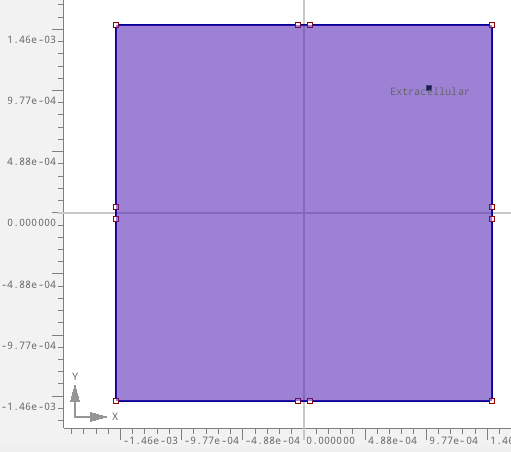
\includegraphics[width=\textwidth]{FE_structure}
            \caption{Electrode and Extracellular Configuration}
            \label{fig:FE_structure}
        \end{minipage}
        \hfill
        \begin{minipage}[b]{0.3\textwidth}
            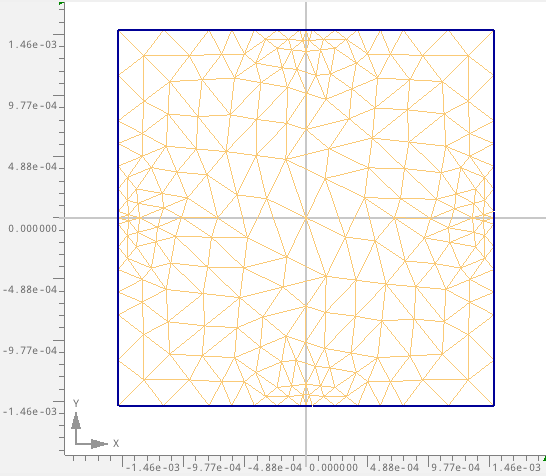
\includegraphics[width=\textwidth]{FE_mesh_1}
            \caption{Generated Mesh for Finite Element Simulation}
            \label{fig:FE_mesh_1}
        \end{minipage}
        \hfill
        \begin{minipage}[b]{0.3\textwidth}
            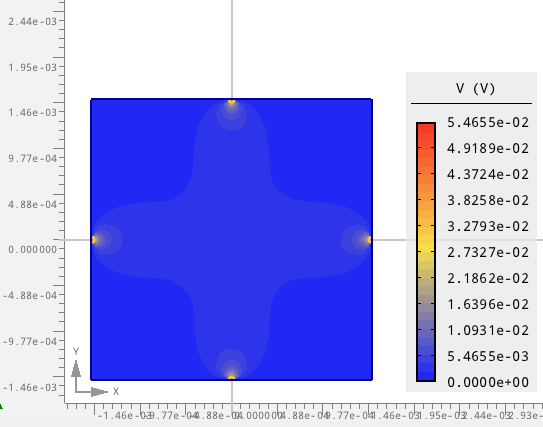
\includegraphics[width=\textwidth]{FE_efield_1}
            \caption{Calculated E-Field for the given Configuration}
            \label{fig:FE_efield_1}
        \end{minipage}
    \end{figure}

    Looking at Figure \ref{fig:FE_efield_at_electrode_1} we see though, that especially for sharp changes in the electrical potential there are issues with the accuracy of this result.

    \begin{figure}[htbp]
        \centering
        \begin{minipage}[b]{0.49\textwidth}
            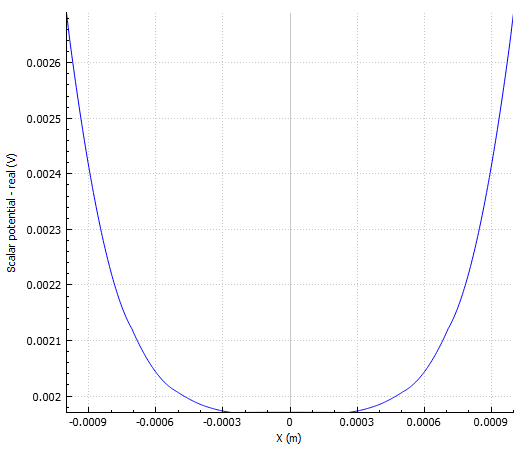
\includegraphics[width=\textwidth]{FE_efield_along_fiber_1}
            \caption{ along the fiber in the center of the chamber}
            \label{fig:FE_efield_along_fiber_1}
        \end{minipage}
        \hfill
        \begin{minipage}[b]{0.49\textwidth}
            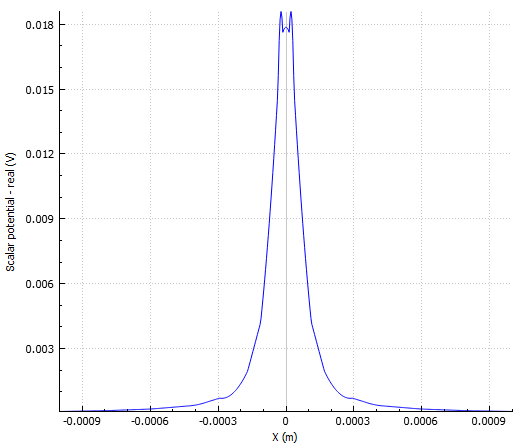
\includegraphics[width=\textwidth]{FE_efield_at_electrode_1}
            \caption{Electrical potential near the upper electrode}
            \label{fig:FE_efield_at_electrode_1}
        \end{minipage}
    \end{figure}

    \subsection{}

    Next we increase the refinement iterations of the mesh to 2 and 3.
    The results can be seen in Figure \ref{fig:FE_mesh_1_1}-\ref{fig:FE_efield_at_electrode_3}.
    As we can see, the mesh gets more dense for each added iteration, also the results for the electrical potential are already a lot better for two iterations.

    \begin{figure}[htbp]
        \centering
        \begin{minipage}[b]{0.3\textwidth}
            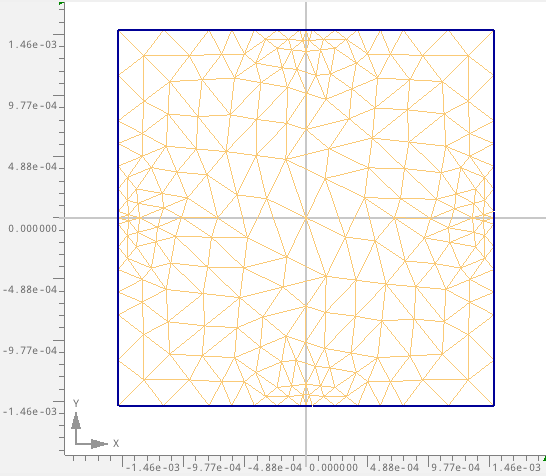
\includegraphics[width=\textwidth]{FE_mesh_1}
            \caption{Generated Mesh for 1 refinement iteration}
            \label{fig:FE_mesh_1_1}
        \end{minipage}
        \hfill
        \begin{minipage}[b]{0.3\textwidth}
            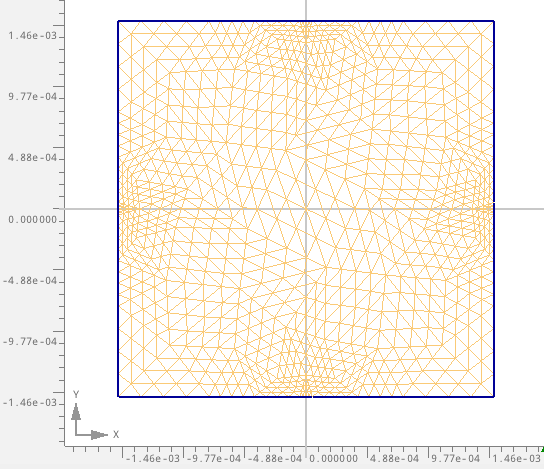
\includegraphics[width=\textwidth]{FE_mesh_2}
            \caption{Generated Mesh for 2 refinement iterations}
            \label{fig:FE_mesh_2}
        \end{minipage}
        \hfill
        \begin{minipage}[b]{0.3\textwidth}
            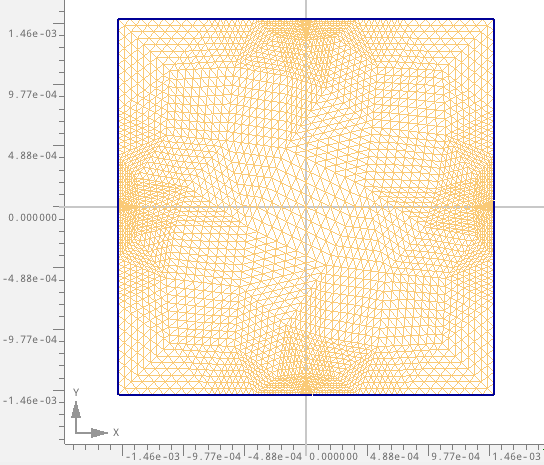
\includegraphics[width=\textwidth]{FE_mesh_3}
            \caption{Generated Mesh for 2 refinement iterations}
            \label{fig:FE_mesh_3}
        \end{minipage}
    \end{figure}

    \begin{figure}[htbp]
        \centering
        \begin{minipage}[b]{0.3\textwidth}
            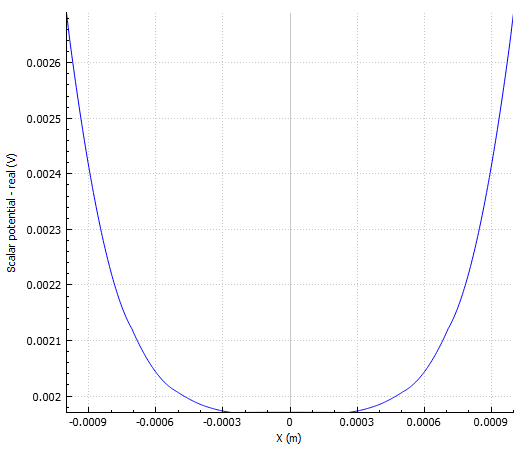
\includegraphics[width=\textwidth]{FE_efield_along_fiber_1}
            \caption{Electrical potential along the fiber for 1 refinement iteration}
            \label{fig:FE_efield_along_fiber_1_1}
        \end{minipage}
        \hfill
        \begin{minipage}[b]{0.3\textwidth}
            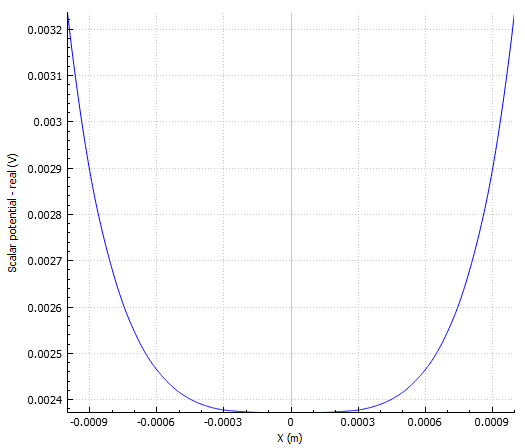
\includegraphics[width=\textwidth]{FE_efield_along_fiber_2}
            \caption{Electrical potential along the fiber for 2 refinement iterations}
            \label{fig:FE_efield_along_fiber_2}
        \end{minipage}
        \hfill
        \begin{minipage}[b]{0.3\textwidth}
            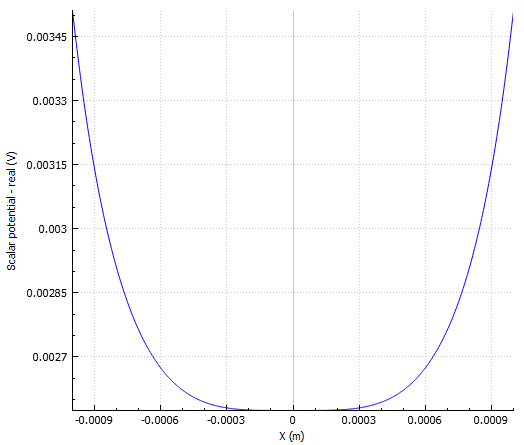
\includegraphics[width=\textwidth]{FE_efield_along_fiber_3}
            \caption{Electrical potential along the fiber for 3 refinement iterations}
            \label{fig:FE_efield_along_fiber_3}
        \end{minipage}
    \end{figure}

    \begin{figure}[htbp]
        \centering
        \begin{minipage}[b]{0.3\textwidth}
            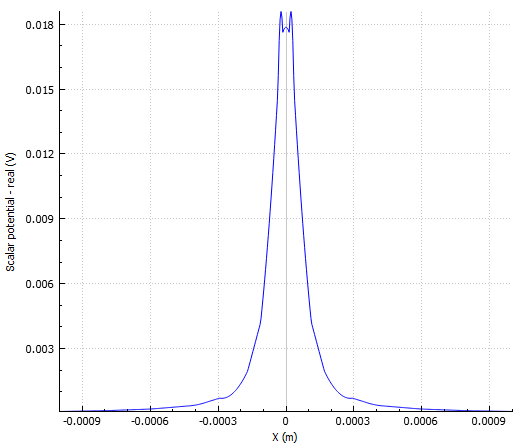
\includegraphics[width=\textwidth]{FE_efield_at_electrode_1}
            \caption{Electrical potential near the upper electrode for 1 refinement iteration}
            \label{fig:FE_efield_at_electrode_1_1}
        \end{minipage}
        \hfill
        \begin{minipage}[b]{0.3\textwidth}
            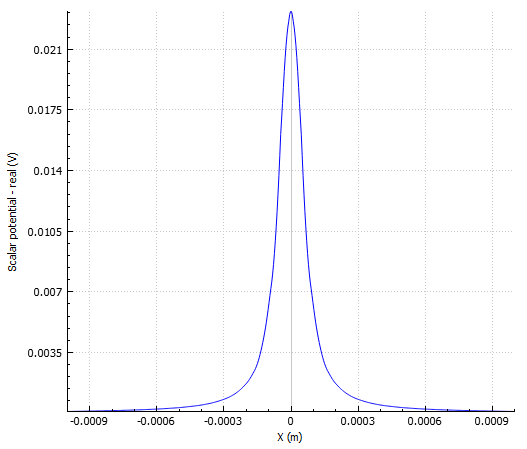
\includegraphics[width=\textwidth]{FE_efield_at_electrode_2}
            \caption{Electrical potential near the upper electrode for 2 refinement iterations}
            \label{fig:FE_efield_at_electrode_2}
        \end{minipage}
        \hfill
        \begin{minipage}[b]{0.3\textwidth}
            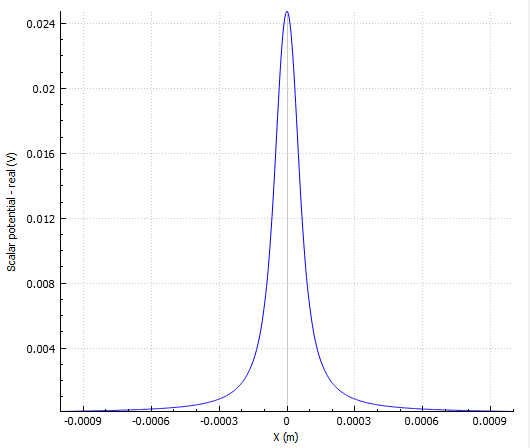
\includegraphics[width=\textwidth]{FE_efield_at_electrode_3}
            \caption{Electrical potential near the upper electrode for 3 refinement iterations}
            \label{fig:FE_efield_at_electrode_3}
        \end{minipage}
    \end{figure}

    \subsection{}

    The following results show the anodic and cathodic spiking threshold for the electrode configuration above

    \begin{enumerate}
        \item \textbf{Direct Scaling}: Potentials imported in \texttt{HH\_multi.py} were scaled by the stimulus amplitude $I$. The calculated thresholds for this method were as follows:
        \begin{align*}
            \text{Cathodic Threshold} &: -50 \\
            \text{Anodic Threshold} &: 180
        \end{align*}

        \item \textbf{Electrode Boundary Condition Modification}: The stimulus current $I$ was set to $1\mu A$, and the applied current density was directly modified in \texttt{Agros2D} by altering the electrode boundary condition. The calculated current densities and corresponding thresholds were as follows:
        \begin{align*}
            \text{Cathodic Threshold} &: -50 \text{ (Current Density} = -6369.43\mu A/mm^2) \\
            \text{Anodic Threshold} &: 180 \text{ (Current Density} = 22929.94\mu A/mm^2)
        \end{align*}
    \end{enumerate}

    As we can see both methods yield the exact same results, which was to be expected since the scaling of the current is of linear nature.
    This outcome is expected since the action potentials scale linearly with stimulus amplitude.

    \subsection{}

    The following shows the spiking threshold for different electrode configurations depicted in Figure \ref{fig:FE_efield_1_1}-\ref{fig:FE_efield_vertical}:

    \begin{enumerate}
        \item \textbf{Four electrodes}:
        \begin{align*}
            \text{Cathodic Threshold} &: -50 \\
            \text{Anodic Threshold} &: 180
        \end{align*}
        \item \textbf{Horizontally aligned electrodes}:
        \begin{align*}
            \text{Cathodic Threshold} &: -40 \\
            \text{Anodic Threshold} &: 120
        \end{align*}

        \item \textbf{Vertically aligned electrodes}:
        \begin{align*}
            \text{Cathodic Threshold} &: -200 \\
            \text{Anodic Threshold} &: 100
        \end{align*}
    \end{enumerate}

    Figures \ref{fig:FE_all_anodic_loc}-\ref{fig:FE_vertical_cathodic_loc} depict the location where the action potential initiates for each given configuration and for an anodic and a cathodic impulse.
    Those result seem correct, considering the proximity of the electrodes as well as, the fact, that anodic impulses tend to induce action potentials further away from the electrode, whereas cathodic impulses stimulate directly next to them.

    \begin{figure}[htbp]
        \centering
        \begin{minipage}[b]{0.3\textwidth}
            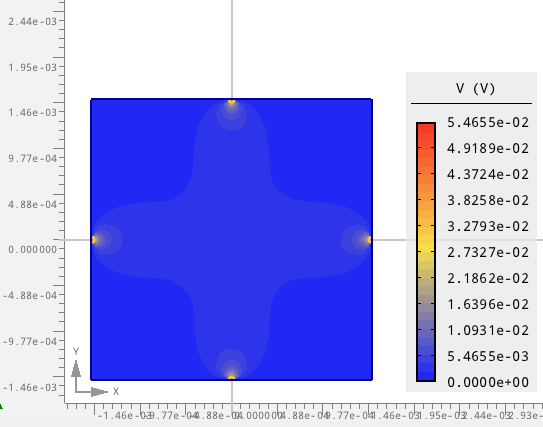
\includegraphics[width=\textwidth]{FE_efield_1}
            \caption{Calculated E-Field for four electrodes}
            \label{fig:FE_efield_1_1}
        \end{minipage}
        \hfill
        \begin{minipage}[b]{0.3\textwidth}
            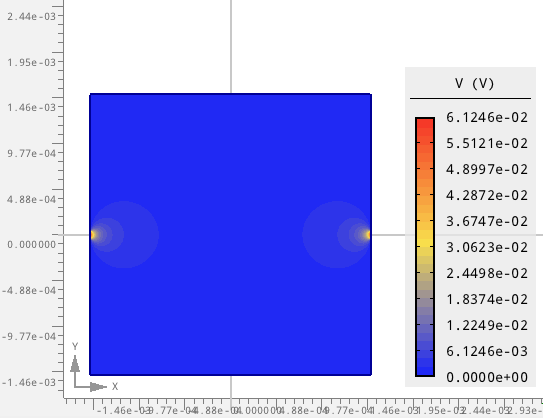
\includegraphics[width=\textwidth]{FE_efield_horizontal}
            \caption{Calculated E-Field for two horizontally aligned electrodes}
            \label{fig:FE_efield_horizontal}
        \end{minipage}
        \hfill
        \begin{minipage}[b]{0.3\textwidth}
            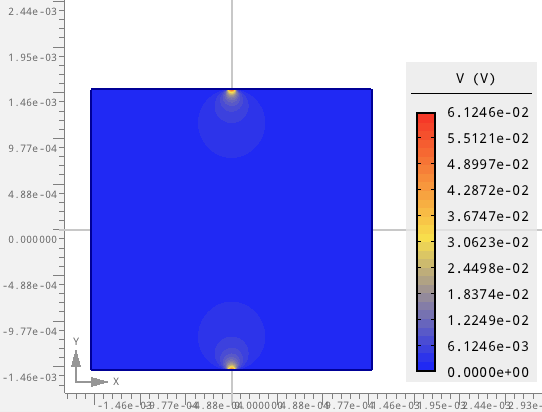
\includegraphics[width=\textwidth]{FE_efield_vertical}
            \caption{Calculated E-Field for two vertically aligned electrodes}
            \label{fig:FE_efield_vertical}
        \end{minipage}
    \end{figure}

    \begin{figure}[htbp]
        \centering
        \begin{minipage}[b]{0.3\textwidth}
            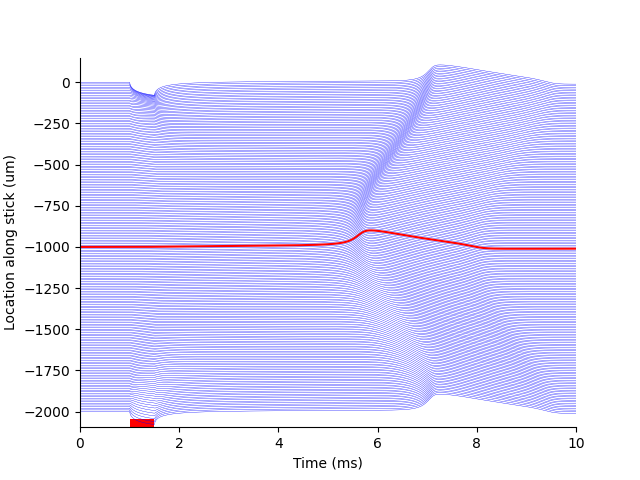
\includegraphics[width=\textwidth]{FE_all_anodic_loc}
            \caption{Anodic action potential initialization location for four electrodes}
            \label{fig:FE_all_anodic_loc}
        \end{minipage}
        \hfill
        \begin{minipage}[b]{0.3\textwidth}
            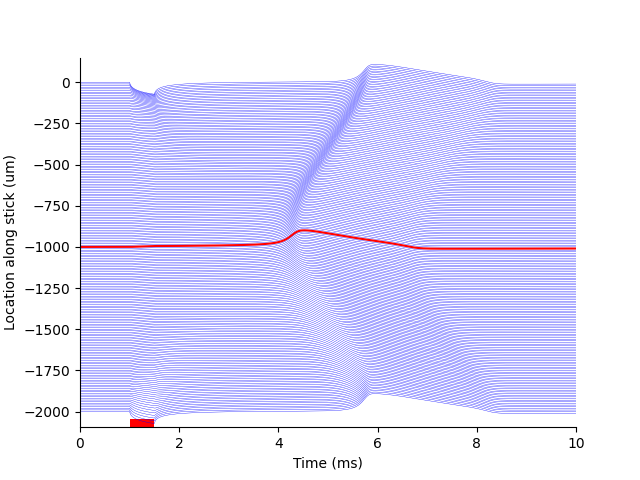
\includegraphics[width=\textwidth]{FE_horizontal_anodic_loc}
            \caption{Anodic action potential initialization location for two horizontally aligned electrodes}
            \label{fig:FE_horizontal_anodic_loc}
        \end{minipage}
        \hfill
        \begin{minipage}[b]{0.3\textwidth}
            \includegraphics[width=\textwidth]{FE_vertical_anodic_loc}
            \caption{Anodic action potential initialization location for two vertically aligned electrodes}
            \label{fig:FE_vertical_anodic_loc}
        \end{minipage}
    \end{figure}

    \begin{figure}[htbp]
        \centering
        \begin{minipage}[b]{0.3\textwidth}
            \includegraphics[width=\textwidth]{FE_all_cathodic_loc}
            \caption{Cathodic action potential initialization location for four electrodes}
            \label{fig:FE_all_cathodic_loc}
        \end{minipage}
        \hfill
        \begin{minipage}[b]{0.3\textwidth}
            \includegraphics[width=\textwidth]{FE_horizontal_cathodic_loc}
            \caption{Cathodic action potential initialization location for two horizontally aligned electrodes}
            \label{fig:FE_horizontal_cathodic_loc}
        \end{minipage}
        \hfill
        \begin{minipage}[b]{0.3\textwidth}
            \includegraphics[width=\textwidth]{FE_vertical_cathodic_loc}
            \caption{Cathodic action potential initialization location for two vertically aligned electrodes}
            \label{fig:FE_vertical_cathodic_loc}
        \end{minipage}
    \end{figure}


\end{document}
